\chapter{Modélisation cinétique}
\label{ch:modelisation_cinetique}

\vfill

Ce dernier chapitre est consacré à la simulation des processus cinétiques ayant lieu dans les atmosphères à base de \ch{C2H2} et \ch{NH3} étudiées Chapitre~\ref{ch:caracterisation_atmospheres} et leur simplification pour une utilisation dans des schémas numériques de volumes finis, de Boltzmann sur réseau, etc. Cela vise à rendre possible la simulation des écoulements réactifs des atmosphères utilisées dans les traitements thermochimiques de cémentation, nitruration et carbonitruration à basse pression. On cherche dans un premier temps à vérifier la pertinence de certains mécanismes cinétiques rapportés dans la littérature pour la simulation de la décomposition des précurseurs \ch{C2H2}~\cite{Norinaga2009} et \ch{NH3}~\cite{Dirtu2006}, et on utilisera nos résultats expérimentaux pour la validation des simulations. Sachant que l'état d'avancement de la pyrolyse de l'acétylène n'est pas très important à basse pression pour des temps de séjour de l'ordre d'une dizaine de
secondes, on se servira de la méthode des \og{}graphes orientés\fg{} (DRG) pour éliminer certaines espèces du mécanisme cinétique de \citet{Norinaga2009}. Cela rend possible la simulation des réacteurs industriels de cémentation avec des temps de calcul raisonnables tout en conservant l'aspect quantitatif de la simulation des espèces majoritaires dans le système \textemdash{} hydrocarbures légers. L'approche DRG de \citet{Lu2005} est utilisée dans ce but. Elle permet l'obtention de \og{}mécanismes squelettes\fg{} dans l'espace des phases échantillonné avant simplification. On commence Section~\ref{sec:modeles-reacteur} avec une bref description des modèles de réacteur et de mélange utilisés \textendash{} réacteur de type parfaitement agité, réacteur de type piston et modèle de mélange complet \textendash{} et de leurs applications. Puis, les mécanismes cinétiques adoptés pour les simulations sont présentés
Section~\ref{sec:mecanismes-cinetiques}. Ensuite, le mécanisme de pyrolyse de l'acétylène est simplifié pour les conditions de la cémentation à basse pression Section~\ref{sec:simplification-mechanisme}. On termine Section~\ref{sec:integration-mecanismes} avec l'intégration des processus cinétiques et avec la comparaison des résultats ainsi obtenus avec des données expérimentales présentées Chapitre~\ref{ch:caracterisation_atmospheres}. Cela permettra d'illustrer l'influence des conditions opératoires sur la décomposition des précurseurs étudiés et de valider l'emploi de ces mécanismes pour décrire les traitements thermochimiques.

\vfill\clearpage

\section{Modèles de réacteur et de mélange}
\label{sec:modeles-reacteur}

Avant de procéder à l'intégration des processus cinétiques et à la présentation des mécanismes choisis pour la simulation de l'évolution des atmosphères étudiées, un modèle de réacteur doit être adopté. Ce choix est basé dans des aspects géométriques, hydrodynamiques et thermiques/thermochimiques. De manière plus générale la simulation des écoulements réactifs peut être réalisée en utilisant des méthodes comme les volumes finis ou de type Boltzmann sur réseau, ce qui peut nécessiter un gros effort de calcul numérique. Pour des géométries simples comme celles des réacteurs tubulaires employés dans cette étude (Figure~\ref{fig:experimental_system}) quelques simplifications sont possibles, rendant les simulations beaucoup plus rapides. Tout d'abord, on vérifie le caractère laminaire de l'écoulement à partir du nombre de Reynolds, ce qui a été réalisé Section~\ref{sec:caracterization_gaz} pour le réacteur à pression atmosphérique. Ce résultat reste valable à basse pression étant donné que les débits massiques et les viscosités similaires sont accompagnés d'une réduction importante de l'inertie \textendash{} introduit par la masse spécifique \textendash{} en raison de la pression utilisée qui est de l'ordre de 5\% de la pression atmosphérique. Cette condition est requise pour éviter d'utiliser une méthode prenant en compte les fluctuations introduites par le régime turbulent et on procède à une présentation de quelques uns des modèles possibles de réacteur. 

Dans ce qui suit, l'idée d'un modèle de réacteur tubulaire à flux laminaire n'a pas été retenue en raison de la discrétisation 2D que cela nécessite, et qui est trop gourmande en temps de calcul. Pour des conditions où le transport par diffusion dans la direction axiale peut être négligé \textendash{} conditions favorisées par des temps de séjour courts, de l'ordre de \SI{1}{\second} pour les gaz \textendash{} le comportement de réacteur de type piston peut suffire et conduire à un gain de temps considérable. La principale origine des écarts introduits par cette description simplifiée est associée au front parabolique de vitesses du fluide. En raison de l'absence de mesures de temps de séjour à basse pression dans notre étude, le système (Figure~\ref{fig:reacteur_bp}) est considéré comme étant de type piston du fait des similitudes avec les conditions employées par \citet{Becker1998177} et des temps de séjour de l'ordre de \SI{1}{\second} que nous avons pu estimer dans nos conditions opératoires. La loi des gaz parfaits ($\rho=\nicefrac{PM}{RT}$, Équation~\ref{eq:ideal_gas_law}) est adoptée comme équation d'état pour toutes les simulations réalisées. Les modèles décrits ci-après interviennent dans la façon dont les équations de conservation de la masse, des espèces et de l'énergie sont posées et une description détaillée est fournie dans des ouvrages de référence~\cite{Himmelblau1997,Fogler1999,Kee2003} ainsi que dans la documentation de la bibliothèque de fonctions Cantera~\cite{Cantera2014} utilisée dans cette étude. Le Tableau~\ref{tab:modeles-reactor} présente une liste des modèles employés au cours de ce chapitre.

\begin{table}[h]
  \caption{\label{tab:modeles-reactor}Modèles de réacteur et de mélange utilisés dans ce chapitre.}
  
  \centering{}\footnotesize{}
  \begin{tabular}{\$l^l}
    \toprule[2pt]
    \rowstyle{\bfseries}
    Modèle 
    & Objectifs
    \tabularnewline
    \midrule[2pt]
    Réacteur parfaitement agité 
    & Analyse de sensibilité/simplification des mécanismes
    \tabularnewline
    Mélange complet 
    & Prédiction des taux de conversion après mesure de $E(t_{s})$
    \tabularnewline
    Réacteur piston 
    & Conversion dans un réacteur laminaire à basse pression
    \tabularnewline
    \bottomrule
  \end{tabular}
\end{table}

\subsection{Réacteur parfaitement agité}
\label{sec:reacteur-agite}

Le plus simple des modèles de réacteur est celui de \og{}réacteur parfaitement agité\fg{} qui décrit une cinétique zéro-dimensionnelle. Si l'on considère seulement le cas des réacteurs ouverts, un tel réacteur est composé d'une chambre traversée par des débits de précurseurs. L'hypothèse fondamentale de cette description est une homogénéité chimique et thermique du volume décrit: le réacteur est isotherme et tout élément de gaz arrivant dans la chambre de réaction est dilué instantanément dans le contenu de l'enceinte. Un réacteur parfaitement agité peut être traité à pression constante, en décrivant les changements de volume qu'il établit en fonction de la température ou des variations des quantités de particules dans le réacteur. Une description est également possible à volume constant. Ce comportement de mélange apparait pour certaines conditions d'injection de gaz dans la chambre, comme dans le cas d'un jet de gaz entrant en collision avec les parois qui serait aussi forcé à se mélanger rapidement \textendash{} par rapport au temps de séjour \textendash{} avec le contenu présent. Des solutions analytiques peuvent être dérivées~\cite{Fogler1999} dans certains cas avec un nombre limité d'espèces \textendash{} généralement inférieur à quatre \textendash{} mais ici on s'en tiendra à leur intégration numérique à l'aide de Cantera~\cite{Cantera2014}, donc en faisant avancer dans le temps la composition du gaz et les variables d'état indépendantes. Même si un tel modèle est fondamentalement théorique et d'usage très limité, sa simplicité rend possible son utilisation dans l'analyse de schémas cinétiques soit en termes de sensibilité~\cite{Turanyi1989} soit pour l'obtention de systèmes simplifiés.

\subsection{Mélange complet}
\label{sec:micromelange-complet}

Le modèle de mélange complet introduit par \citet{Zwietering1959} permet la description des réacteurs à faible nombre de Bodenstein et ayant une distribution de temps de séjour quelconque. Il est utile pour des conditions dans lesquelles la mise en solution avec des éléments de volume arrivant dans le réacteur est supposée instantanée dans des volumes \og{}d'âges\fg{}  différents. Ce modèle pondère la dilution d'un volume à l'intérieur du réacteur ayant une espérance de vie $\lambda$ avec les nouveaux éléments arrivant par la fonction densité de probabilité $E(\lambda)\equiv{E(t_{\infty}-t_{s})}$~\cite{Fogler1999,Himmelblau1997}. Génériquement pour le calcul de la concentration $c_{i}$ de l'espèce $i$ à la sortie du réacteur, on écrit l'Équation~\ref{eq:maximum_mixedness}, qui représente un modèle de réacteur de type agité. La variable indépendante de ce modèle dynamique n'est pas le temps, mais l'espérance de vie $\lambda$ des éléments de volume du gaz à l'intérieur du réacteur, espérance qui vaut zéro à la sortie du réacteur. Les autres symboles ont déjà été définis dans le texte. L'utilisation de ce modèle, qui représente le cas limite opposé à celui de la ségrégation ($Bo{}\geq{}50$)~\cite{Becker1998177,Fogler1999} lequel considère qu'aucune dilution des nouveaux éléments arrivant au réacteur n'a lieu, est assez simple et sert à estimer la conversion en sortie d'un réacteur si le changement de volume molaire produit par les transformations chimiques n'est pas important.

\begin{equation}
\frac{\mathrm{d}c_{i}}{\mathrm{d}\lambda}=
-\dot{\omega}_{i}+(c_{i}-c_{i,0})\frac{E(\lambda)}{1-F(\lambda)}
\label{eq:maximum_mixedness}
\end{equation}

L'intégration de l'Équation~\ref{eq:maximum_mixedness} ne peut pas se faire directement en fonction de la variable $\lambda$, ce qui demanderait une intégration dans le temps de $t_{\infty}$ à zéro. En pratique, le temps infini adopté est un temps $t_{max}$ suffisamment grand par rapport à $t_{\infty}$ expérimental pour tenir compte des contributions des éléments de volume les plus anciens dans l'enceinte. On adopte typiquement une valeur $t_{max}$ telle que $F\left(t_{max}\right)\approx{}0,9999$ pour des raisons de stabilité numérique. Grâce au changement de variable $\lambda=t_{max}-t$, on écrit l'Équation~\ref{eq:maximum_mixedness_num} qui est ensuite intégrée dans l'intervalle de temps $t=(0;t_{max})$. Le paramètre $c_{i,0}$ correspond à la concentration de l'espèce $i$ du mélange injecté dans le réacteur et c'est sa mise en solution avec les éléments à l'intérieur du réacteur qui est pondérée par $E(\lambda)$.

\begin{equation}
\frac{\mathrm{d}c_{i}}{\mathrm{d}t}=
-\biggr[\dot{\omega}_{i}+(c_{i}-c_{i,0})\frac{E(t_{max}-t)}{1-F(t_{max}-t)}\biggr]
\label{eq:maximum_mixedness_num}
\end{equation}

\subsection{Réacteur piston}
\label{sec:reacteur-piston}

Les réacteurs tubulaires à écoulement laminaire peuvent être le siège d'un transport par diffusion axiale important sous certaines conditions. Lorsqu'on réduit la pression de travail $P_{op}$, pour un débit massique à l'entrée fixe dans un réacteur à section constante, la vitesse moyenne $u$ de l'écoulement augmente selon le rapport $P_{ref}/P_{op}$, où $P_{ref}$ représente la pression de départ \textendash{} ou de référence. Lorsque $u$ augmente, le nombre de Reynolds $Re$ reste pratiquement inchangé en raison de l'évolution inverse de la densité \textemdash{} les effets visqueux étant négligés. Dans ce scénario, l'augmentation de la vitesse mène à une réduction du nombre de Peclet (Équation~\ref{eq:bodenstein_peclet}) et donc à une diminution du degré de mélange dans la direction de l'axe du réacteur: on peut négliger le transport par diffusion dans cette direction lorsque $Pe_{ax}\rightarrow{}0$. Ce modèle suppose dans le cas le plus simple, en l'absence de réactions de surface, la conservation du flux massique ($\dot{m}=\rho uA_{c}$) selon la direction de l'axe du réacteur, Équation~\ref{eq:mass_continuity_no_wall_term}, où $A_{c}$ est la section transversale de l'écoulement, $\rho$ la masse volumique et $u$ la vitesse axiale. Des généralisations comprenant des processus de surface sont fournies par \citet{Khan2008} et \citet{Deutschmann2001}. Autrement dit, $\rho{}u$ est constant: masse volumique et vitesse sont couplées par une équation algébrique issue de la condition imposée par l'Équation~\ref{eq:mass_continuity_no_wall_term}.

\begin{equation}
A_{c}\frac{\mathrm{d}\left(\rho u\right)}{\mathrm{d}t}=0
\label{eq:mass_continuity_no_wall_term}
\end{equation}

Ce modèle prédit la conversion à l'état stationnaire en un endroit quelconque du réacteur où l'équilibre entre le transfert de chaleur sur les parois, l'apport en énergie par des réactions chimiques et le transport convectif prévaut. Cela se fait par l'Équation~\ref{eq:energy_balance_convection}, où $c_{P}$ est la chaleur spécifique du mélange, $U$ le coefficient global de transfert de chaleur, $T_{p}$ la température de la paroi. Le second terme à gauche représente une source de génération de chaleur par voie chimique $S_{ch}$. 

\begin{equation}
\rho uA_{c}\frac{\mathrm{d}\left(c_{P}T\right)}{\mathrm{d}z}+A_{c}S_{ch}=
UA_{s}\left(T_{p}-T\right)
\label{eq:energy_balance_convection}
\end{equation}

Cette approche est équivalente à considérer que le réacteur tubulaire est composé d'une série de \og{}tranches\fg{} de réacteurs agités de longueur différentielle à l'état stationnaire. C'est à partir de cette formulation qu'on peut simuler des réacteurs de comportement piston à l'aide de Cantera~\cite{Cantera2014}: la longueur du tube est divisée en un nombre $N_{r}$ de réacteurs parfaitement agités de volume $V=A_{c}\cdot{\mathrm{d}z}$. Le premier réacteur de la chaine est amené à l'état stationnaire et la composition obtenue est utilisée comme donnée d'entrée pour le réacteur suivant et cela sur toute la longueur du réacteur. Pour incorporer les transferts thermiques, on suppose que le nombre de Nusselt $Nu\approx{}4$~\cite{Incropera2011}, condition intermédiaire entre une température et un flux d'énergie imposés sur les parois. En négligeant la conduction vers le milieu extérieur, on obtient $U\approx{}4k_{g}D^{-1}$, où $k_{g}$ est la conductivité thermique moyenne du gaz et $D$ le diamètre du tube. La conductivité thermique $k_{g}$ est calculée en considérant un comportement de mélange parfait et en utilisant les conductivités $k_i$ de chaque espèce présente calculées à partir des paramètres de Lennard-Jones~\cite{Bird}.

\section{Mécanismes cinétiques}
\label{sec:mecanismes-cinetiques}

La simulation des écoulements réactifs se fait en partant d'un mécanisme cinétique comprenant les réactions chimiques principales et leurs vitesses de réaction respectives. Ces vitesses peuvent être empiriques ou issues de simulations théoriques~\cite{Henriksen2008}. Elles sont généralement paramétrées par une loi exponentielle modifiée de type Arrhenius. Ces données permettent le calcul des vitesses de réaction, c'est-à-dire de formation/consommation des espèces chimiques. La Section~\ref{sec:cinetique} a présenté les fondements de la cinétique chimique selon la loi d'action de masse et introduit quelques modifications souvent utilisées pour décrire des effets de pression. Un modèle simple de réacteur tout comme un calcul de dynamique des fluides (CFD, LBM, etc) permet le couplage entre phénomènes chimiques \textendash{} changement de composition et échanges thermiques \textendash{} et écoulement dans l'enceinte du réacteur \textemdash{} comportement de mélange, distribution des espèces, changement de vitesse, etc. L'établissement d'un schéma cinétique étant une tâche très longue, généralement de plusieurs années en raison de l'introduction successive de processus cinétiques de plus en plus fins améliorant les mécanismes principaux, on se contentera de présenter des schémas issus de la littérature utilisés pour simuler des écoulements réactifs à base d'hydrocarbures d'abord et d'ammoniac ensuite. Les mécanismes de référence adoptés ont leurs nombres d'espèces et de réactions présentés Tableau~\ref{tab:kinetic-mecanisms}. Ces schémas n'ont pas été reproduits ici car nous avons utilisé exactement les mêmes que ceux des publications citées. Il suffit donc de s'y référer pour avoir la description exhaustive des réactions et des constantes cinétiques utilisées.

\begin{table}[!t]
  \caption{\label{tab:kinetic-mecanisms}Mécanismes cinétiques utilisés dans la simulation de la pyrolyse de l'acétylène et de la décomposition de l'ammoniac.}
  
  \centering{}\footnotesize{}
  \begin{tabular}{\$c^c^c^c}
    \toprule[2pt]
    \rowstyle{\bfseries}
    Précurseur 
    & Nombre d'espèces
    & Nombre de réactions 
    & Références
    \tabularnewline
    \midrule[2pt]
    \ch{C2H2} 
    & 241 (gaz) 
    & 902 (gaz) 
    & \citet{Norinaga2009}
    \tabularnewline[6pt]
    \multirow{2}{2cm}{\centering \ch{NH3}} 
    & 10 (gaz) 
    & 19 (gaz) 
    & \multirow{2}{3cm}{\centering \citet{Dirtu2006}} 
    \tabularnewline
    & 1 (surface) 
    & 2 (surface) 
    &
    \tabularnewline
    \bottomrule
  \end{tabular}
\end{table}

\subsection{Mécanisme de pyrolyse de l'acétylène}
\label{sec:mecanisme-acetylene}

Pour la simulation de la pyrolyse de l'acétylène, un mécanisme attribué à \citet{Norinaga2009} a été choisi en fonction de la plage de températures et de pressions utilisées par les auteurs dans leurs études numériques et expérimentales. Ce mécanisme contient 902 réactions et 241 espèces chimiques et résulte d'une compilation de données cinétiques publiées pendant plus de 40 ans dans la littérature. Les auteurs~\cite{Norinaga2009} ont traité la pyrolyse de l'acétylène ainsi que celle de l'éthylène et du propane dans une série de publications~\cite{Norinaga2005,Norinaga2007,Norinaga2007ii,Norinaga2009} au cours de la dernière décennie, validant le modèle dans la plage de pressions au--dessous de \SI{20}{\hecto\pascal} pour le \ch{C2H2} à \SI{1173}{\kelvin} et pour des temps de séjour de l'ordre de \SI{2}{\second}. \citet{Khan2008} utilise ce mécanisme~\footnote{En fait l'auteur~\cite{Khan2008} emploie une version précédente publiée par \citet{Norinaga2007}.} dans des conditions similaires de pressions partielles à celles de notre étude mais sous une pression totale de \SI{1600}{\hecto\pascal}. L'auteur~\cite{Khan2008} rappelle l'importance de la prise en compte de \ch{CH3COCH3} et de ses dérivés, comme le soulignent aussi \citet{Dimitrijevic2000}, la présence d'acétone dans les bouteilles permettant de stabiliser l'acétylène~\footnote{Des bouteilles de \ch{C2H2} sans acétone sont aussi disponibles.}. 

Un mécanisme simplifié rapporté dans la littérature par \citet{Graf2007} est disponible pour l'acétylène dilué. Ce modèle a été développé pour la modélisation de la cémentation à partir de données expérimentales obtenues au--dessus de la pression atmosphérique. Si l'on intègre ce mécanisme sur des temps de séjour assez courts, il fournit des résultats proches de ceux du mécanisme de \citet{Norinaga2009} pour les espèces \ch{C1} et \ch{C2}, comme cela a été montré par \citet{Khan2008}. Dans la présente discussion, il n'y a pas d'intérêt à l'intégrer: on s'intéresse en effet à des mécanismes simplifiés plus compréhensibles et sans ajustement à l'aide des résultats expérimentaux. Cette discussion vise à montrer l'importance de l'obtention de mécanismes simplifiés pour une application donnée: il a donc été choisi de déterminer un mécanisme squelette à partir de celui de \citet{Norinaga2009}, ce qui a pour but de conserver la cohérence thermodynamique du mécanisme \textendash{} les enthalpies de réaction \textendash{} et d'assurer une simplification substantielle dans des conditions connues expérimentalement.

Le mécanisme de \citet{Norinaga2009} a été analysé d'un point de vue topologique \textendash{} la structure des interdépendances entre les espèces \textendash{} pour identifier les plus importantes sans tenir compte des vitesses de réaction, ce qui fait l'objet de la Section~\ref{sec:simplification-mechanisme}. Si l'on construit le graphe d'interaction orienté des espèces du mécanisme, c'est-à-dire en les utilisant comme n{\oe}uds, on peut les classer selon leur degré, à savoir le nombre total d'arêtes à chaque espèce. Ce classement montre les espèces qui interviennent dans les vitesses de réaction pour la formation du plus grand nombre d'autres espèces dans le système \textendash{} celles qui produisent les colonnes les moins creuses dans la matrice jacobienne du système, laquelle a la forme présentée Figure~\ref{fig:matrice_norinaga}~\footnote{Cette matrice d'adjacence associée au mécanisme est creuse et présente une densité de 0,06. Elle permet l'utilisation d'outils numériques optimisés pour la représentation de ce type de matrices dans l'intégration de ce mécanisme.}. Le résultat de cette analyse est fourni Tableau~\ref{tab:graphe_non_dirige} qui indique les 10 espèces les plus connectées dans le mécanisme et inclut toutes les espèces présentes dans le mécanisme simplifié de \citet{Graf2007} à part le carbone solide, utilisé pour représenter les dépôts de carbone. Si l'on exclut les radicaux listés dans le Tableau~\ref{tab:graphe_non_dirige}, on retrouve l'ensemble des espèces du mécanisme simplifié, ce qui est raisonnable étant donné le court temps de vie des radicaux. Indépendamment de leurs vitesses de formation/consommation, ces espèces seront probablement conservées après simplification selon la méthode de \citet{Lu2005} pour intervenir sur un grand nombre d'autres espèces. Pour éliminer ce comportement, il est recommandé d'utiliser la méthode CSP~\cite{Lam1993,Lam1994}, bien que cette technique soit moins intuitive à analyser.

\begin{table}[h]
  \caption{\label{tab:graphe_non_dirige}Classement selon le degré total des espèces les plus connectées dans le mécanisme de \citet{Norinaga2009} et leur degré de connectivité.}
  
  \centering{}\footnotesize{}%
  \begin{tabular}{ccccc}
    \cmidrule[2pt]{1-2} \cmidrule[2pt]{4-5} 
    Espèce      & Degré  &  & Espèce      & Degré \tabularnewline
    \cmidrule[2pt]{1-2} \cmidrule[2pt]{4-5} 
    $\ch{H}$    & 453    &  & $\ch{C2H3}$ & 171    \tabularnewline
    %\cmidrule{1-2} \cmidrule{4-5} 
    $\ch{H2}$   & 408    &  & $\ch{C2H4}$ & 159    \tabularnewline
    %\cmidrule{1-2} \cmidrule{4-5} 
    $\ch{C2H2}$ & 303    &  & $\ch{C6H6}$ & 104    \tabularnewline
    %\cmidrule{1-2} \cmidrule{4-5} 
    $\ch{CH3}$  & 220    &  & $\ch{C6H5}$ & 95     \tabularnewline
    %\cmidrule{1-2} \cmidrule{4-5} 
    $\ch{CH4}$  & 185    &  & $\ch{C4H4}$ & 90     \tabularnewline
    \cmidrule{1-2} \cmidrule{4-5} 
  \end{tabular}
\end{table}

La Figure~\ref{fig:histogramme_norinaga} présente l'histogramme de degré des n{\oe}uds (espèces) du mécanisme de \citet{Norinaga2009}. Sur cette figure, on vérifie qu'il existe un nombre important d'espèces liées à un nombre réduit d'autres espèces \textemdash{} la fréquence maximale est concentrée autour des n{\oe}uds de degré inférieur à 100, le degré ayant le maximum en fréquence étant de 10 pour 50 espèces: environ 20\% des espèces du mécanisme sont couplées à seulement 10 autres espèces. Cette analyse assez rapide a montré le faible degré moyen des n{\oe}uds du système d'équations de ce mécanisme et donc on attend une simplification importante lors de l'utilisation de l'algorithme DRG. Bien que la simulation du mécanisme complet soit lourde en termes de temps de calcul, la connaissance des espèces les plus connectées est une étape importante pour la simplification du mécanisme.% et donc pour l'optimisation du temps de simulation.

\begin{figure}[h]
  \subfloat[\label{fig:histogramme_norinaga}Histogramme]{
    %tex.stackexchange.com/questions/65386
    \raisebox{9mm}{
    \resizebox{0.40\textwidth}{!}{%
    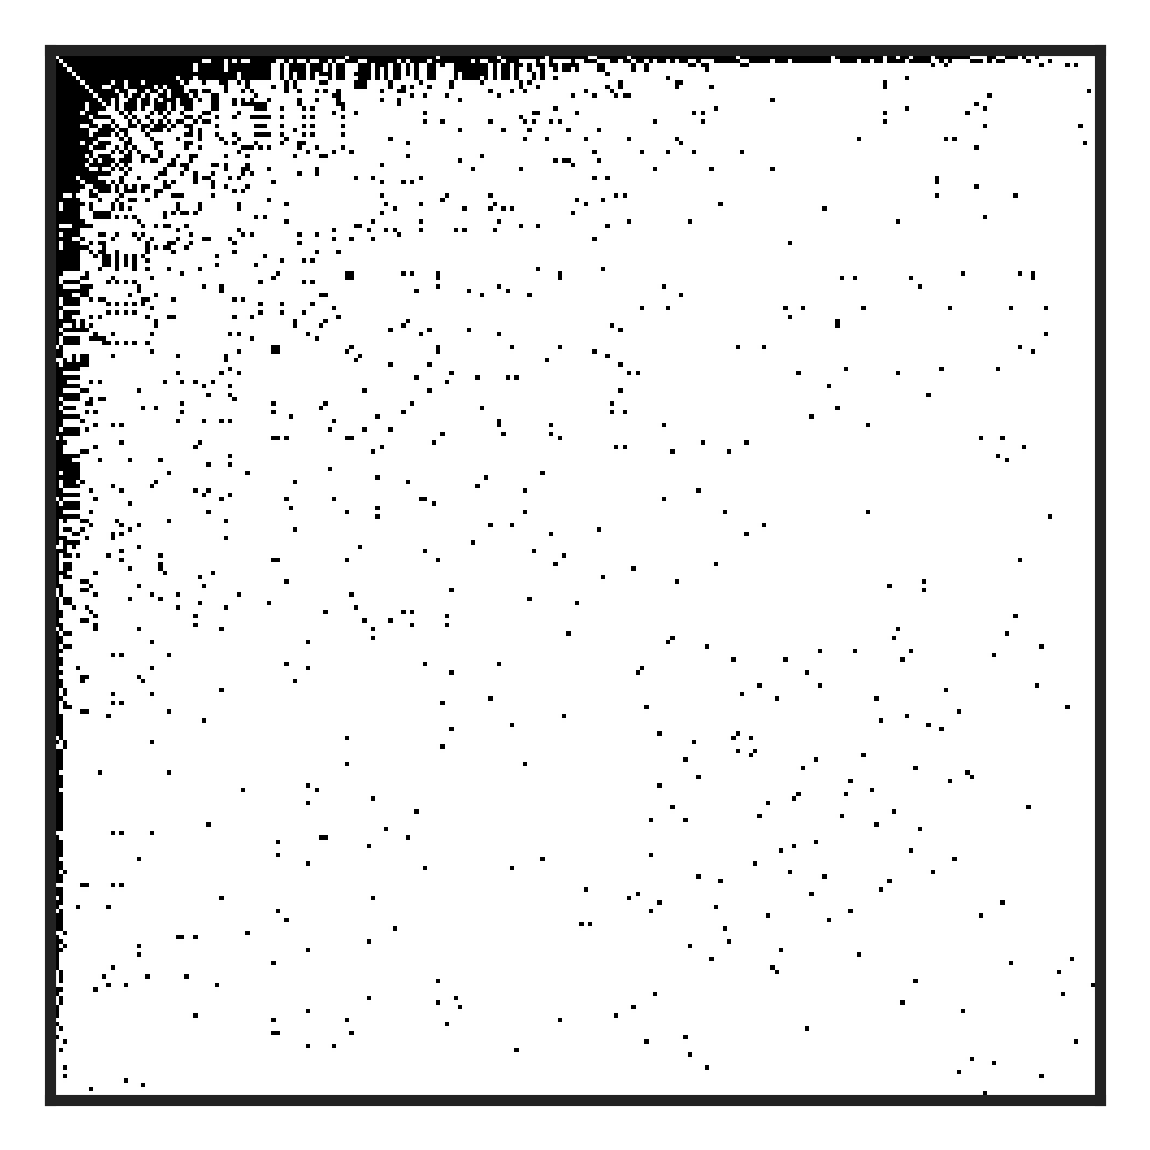
\includegraphics{figures/ch-05-histogram_norinaga-digraph-adjacency}}}
  }\hfill
  \subfloat[\label{fig:matrice_norinaga}Matrice]{
    \resizebox{0.48\textwidth}{!}{%
    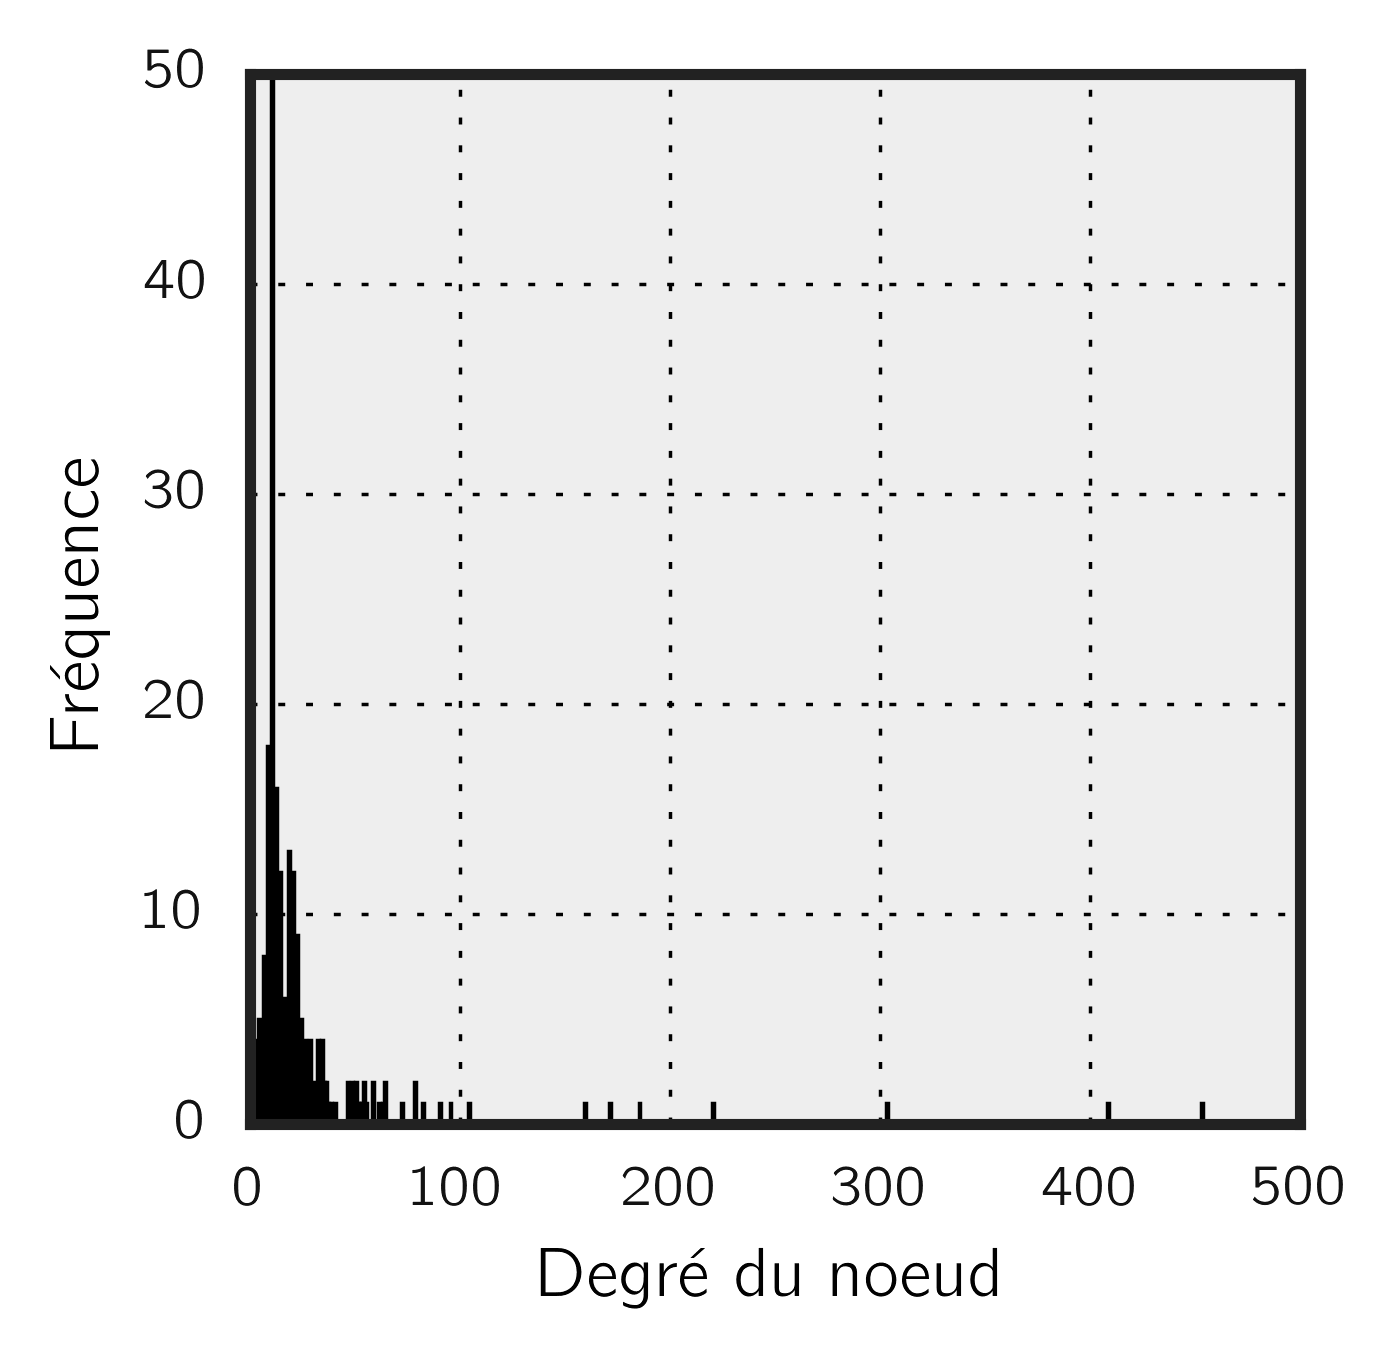
\includegraphics{figures/ch-05-histogram_norinaga-digraph}}
  }

  \caption{Histogramme de degrés des espèces dans le mécanisme de \citet{Norinaga2009} et matrice d'adjacence pour les espèces montrant l'allure de l'occupation de la matrice Jacobienne.}
\end{figure}

\subsection{Mécanisme de décomposition de l'ammoniac}
\label{sec:mecanisme-ammoniac}

Bien que la littérature soit riche en publications relatives à la décomposition des hydrocarbures à basse pression~\cite{Becker1998177,Becker1998201,Becker1998213,Becker1998225,Norinaga2005,Norinaga2007,Norinaga2007ii,Norinaga2009,Khan2008} et propose des compilations de mécanismes qui représentent fidèlement les systèmes de pyrolyse ou de combustion des composants légers, elle s'avère être beaucoup plus pauvre pour l'ammoniac et les espèces du système \ch{N-H}, pour lequel on ne dispose que d'un nombre réduit de données~\cite{Dirtu2006,Odochian2011,Hwang2003,Klippenstein2009} relatives à la cinétique en phase gazeuse dans des conditions d'intérêt pour la nitruration basse pression. En effet, la majorité des résultats sont extrapolés à partir de simulations théoriques des états de transition. L'ammoniac faisant partie de certains processus liés à la combustion, ce précurseur et ses dérivés apparaissent dans des mécanismes~\cite{Grimech,AAUmech} développés dans ce cadre. Ces mécanismes ne sont pas adaptés à une utilisation de \ch{NH3} comme espèce de départ car ils sont plus orientés vers la prédiction des espèces du système \ch{N-O}. 

Les données sur la synthèse de l'ammoniac ne s'avèrent pas utiles aux procédés étudiés en raison des pressions utilisées, \emph{i.e.} la majorité des applications pour la synthèse des composés dérivés de l'ammoniac opèrent à des pressions au--dessus de \SI{1000}{\hecto\pascal} (\SI{1}{\atm}) et les procédés thermochimiques des matériaux utilisant ce précurseur ont été développés principalement à la pression atmosphérique. Une autre raison est la faible vitesse de décomposition homogène de ce précurseur, comme nous l'avons montré Chapitre~\ref{ch:caracterisation_atmospheres}: la décomposition de ce précurseur n'atteint que 6\% à \SI{1173}{\kelvin} et une pression de \SI{100}{\hecto\pascal}.

L'intégration des mécanismes de \citet{Klippenstein2009} ou \citet{Hwang2003} \textendash{} établis à partir de la théorie des états de transition \textendash{} conduit à des niveaux de décomposition négligeables \textendash{} de l'ordre de l'erreur numérique utilisée \textendash{} pour des temps de séjour de l'ordre de \SI{0,5}{\second}, comme celui de nos expériences. Un mécanisme cinétique présenté par \citet{Dirtu2006} et aussi utilisé par \citet{Odochian2011} est la seule compilation de réactions disponible qui permette la simulation des systèmes contenant une fraction importante en ammoniac. Ce mécanisme est composé de 11 espèces chimiques et de 21 réactions \textendash{} certaines étant aussi présentes dans le mécanisme de \citet{AAUmech} \textendash{} dont 2 de surface avec le quartz. 

Le mécanisme de \citet{Dirtu2006} préserve l'ammoniac jusqu'au moment où les radicaux et les espèces minoritaires atteignent une certaine concentration permettant la décomposition de ce précurseur: la rigidité du système cinétique est importante si la composition de départ n'inclut pas de fractions résiduelles \textendash{} c'est-à-dire, des parties par million, selon l'équilibre dans la bouteille \textendash{} de radicaux formés par le mécanisme. Du fait qu'il a été validé avec des résultats expérimentaux~\cite{Dirtu2006,Odochian2011} dans certaines conditions, nous avons choisi le mécanisme de \citet{Dirtu2006} pour la simulation de la phase gazeuse. Des données cinétiques fournies par \citet{Cooper1988} et \citet{Ertl1980} sont incorporées et adaptées pour la simulation des processus de surface. L'introduction d'une densité surfacique de sites actifs sur le quartz fournie par \citet{Tang20151161} permet d'ajuster le craquage de l'ammoniac sur les parois. % du réacteur.

\section{Obtention des mécanismes simplifiés}
\label{sec:simplification-mechanisme}

\subsection{Séquence de simplification}

La simplification des mécanismes cinétiques permet de réduire le nombre d'espèces par élimination de celles dont l'importance est négligeable dans certaines conditions et donc de réduire d'autant l'effort numérique. Il est important que la simplification soit accompagnée d'une validation dans l'espace des états~\footnote{Ici l'espace des états est defini par l'ensemble de variables thermodynamiques indépendantes du système, c'est-à-dire le vecteur $\Phi$ contenant la masse volumique $\rho$, la température $T$ et les fractions molaires $x_{i}$ de toutes les espèces $i$, $\Phi=\{\rho,\,T,\,x_{0},\,x_{1},\,...,\,x_{n}\}$.} d'intérêt pour que l'on puisse incorporer les schémas obtenus dans des problèmes à plus large échelle. Parmi les différents techniques existantes~\cite{Coles2011}, on a choisi d'employer la méthode de \citet{Lu2005} décrite Section~\ref{sec:simplification_cinetique_lu_and_law} en raison de sa simplicité d'implémentation et d'interprétation. La stratégie de simplification du mécanisme de \citet{Norinaga2009} selon cette méthode est composée des étapes suivantes:

\begin{description}[style=unboxed, leftmargin=0cm]
\item[échantillonnage:] l'espace des états du vecteur solution \textendash{} fractions des espèces et variables d'état \textendash{} doit être échantillonné~\footnote{L'étape d'échantillonnage ne possède pas une définition stricte. C'est à l'utilisateur de définir des points représentatifs des compositions qui peuvent être trouvées au cours de l'évolution de l'atmosphère. Il est recommandé d'inclure a minima la composition de départ et les valeurs connues en sortie du réacteur dans l'échantillon de l'espace des états.} de manière à représenter une région connue des compositions obtenues dans l'atmosphère carburante; des solutions utilisant le modèle de réacteur parfaitement agité pour intégrer le mécanisme complet sans tenir compte de l'équation de l'énergie ont été obtenues pour des pressions de \SIlist{10;50;100}{\hecto\pascal} pour l'atmosphère présentée Tableau~\ref{tab:atmosphere-starting}. Pour illustrer le comportement à \SI{1000}{\hecto\pascal} le système a été simplifié pour n'avoir plus que 10\% des fractions des composés du Tableau~\ref{tab:atmosphere-starting}, le diazote représentant 97\% de l'atmosphère;

\begin{table}[h]
  \caption{\label{tab:atmosphere-starting}Composition de départ en fractions molaires pour l'échantillonnage de l'espace des états en vue d'une simplification du mécanisme de \citet{Norinaga2009}.}
  
  \centering{}\footnotesize{}%
  \begin{tabular}{cccc}
    \toprule[2pt] 
    \ch{N2} & \ch{C2H2} & \ch{CH4} & \ch{CH3COCH3}\tabularnewline
    \midrule[2pt] 
    0,700 & 0,294 & 6,0$\times{10^{-4}}$ & 5,4$\times{10^{-3}}$\tabularnewline
    \bottomrule
  \end{tabular}
\end{table}

\item[balayage:] la méthode de \citet{Lu2005} consiste à réaliser une série de simplifications préalables en fonction du paramètre d'erreur $\varepsilon$~\footnote{Ce paramètre ne possède pas un sens physique directe. Sa valeur affecte la proximité entre une intégration d'un mécanisme réduit de celle du mécanisme complet, mais elle n'a aucune relation avec l'erreur relative entre ces intégrations. Des simplifications successives en augmentant la valeur $\varepsilon\in\left[0;\,1\right]$ conduisent typiquement à la diminution du nombre d'espèces dans le mécanisme jusqu'à un seuil contenant les espèces les plus fortement couplées dans l'espace d'états $\phi$ utilisé au départ. Pour rendre notre simplification plus fiable, nous avons choisi de conserver l'union des espèces résiduelles obtenues pour une valeur de $\varepsilon$ pour tous les échantillons $\phi_{i}$ issus des intégrations réalisées pendant l'échantillonnage pour chaque pression utilisée. De cette façon, les espèces conservées dans l'espace des états pour une valeur de $\varepsilon$ donnée sont en fait $N_{\Phi}=\bigcup^{i}N_{\phi_{i}}$, où $N_{\Phi}$ désigne l'ensemble des espèces retenues dans le mécanisme pour une valeur de $\varepsilon$ et $N_{\phi_{i}}$ les espèces retenues pour chaque échantillon $\phi_{i}$ avec la même valeur de $\varepsilon$.} pour identifier les points de découplage interne des sous--graphes~\footnote{Un sous--graphe étant défini comme un graphe $G^{\prime}$ qui fait partie (tous ses n{\oe}uds et toutes ses arêtes) du graphe $G$ représentant l'ensemble des espèces comme des n{\oe}uds. On a donc $G^{\prime}\subseteq{}G$~\cite{Diestel2000}.} composant le système cinétique, ce qui est fait en identifiant dans l'arbre des relations entre espèces les branches associées à la métrique $r_{ij}\geq{}\varepsilon$ \textemdash{} Section~\ref{sec:simplification_cinetique_lu_and_law}. Les régions en échelon (Figure~\ref{fig:diagramme_reduction}) obtenues lors du balayage du mécanisme de \citet{Norinaga2009} selon ce paramètre représentent des valeurs potentielles de $\varepsilon$ pour réaliser la simplification: à 0,06 une chute importante dans le nombre d'espèces est observée pour toutes les pressions, ce qui se répète entre 0,08-0,11, produisant une autre simplification importante; 

\item[composition:] finalement, dans la version la plus simple de la méthode, les mécanismes squelettes sont obtenus par l'union des différentes simplifications obtenues à partir des échantillons de l'espace des états: ces unions ont pour but de générer un mécanisme simplifié qui représente tout l'espace des solutions des échantillons. Dans tous les mécanismes simplifiés, les espèces de départ du Tableau~\ref{tab:atmosphere-starting} et le \ch{C2H4} ont été utilisées comme n{\oe}uds de base dans l'algorithme de parcours en profondeur et sont forcément conservées dans les mécanismes.
\end{description}

\noindent Ces étapes sont détaillées de façon algorithmique ci--dessous:
\begin{itemize}
  \item Échantillonnage (pour chaque pression $P$):
  \begin{inparaenum}[(i)]
    \item intégration des conditions de départ choisies et
    \item enregistrement de quelques états intermédiaires.
  \end{inparaenum}
  \item Balayage (initialiser $\varepsilon=0$):
  \begin{inparaenum}[(i)]
    \item pour chaque point de solution de chaque intégration, simplifier,
    \item enregistrer les espèces à retenir de la simplification et
    \item avancer $\varepsilon$ de $\Delta\varepsilon$ (nous avons utilisé un pas de 0,004).
  \end{inparaenum}
  \item Composition (pour chaque valeur de $\varepsilon$):
  \begin{inparaenum}[(i)]
    \item réaliser l'union de toutes les espèces à retenir pour chaque $\varepsilon$ et
    \item éliminer les espèces redondantes de l'ensemble.
  \end{inparaenum}
\end{itemize}

Il est possible d'ajouter une étape supplémentaire de composition du mécanisme simplifié en utilisant les espèces retenues issues de simplifications réalisées à des différentes pressions et une valeur fixe de $\varepsilon$ pour augmenter la plage de validité du mécanisme squelette. La même chose peut être faite pour la température ou en réalisant une combinaison de paramètres de température et pression.

\subsection{Analyse de la simplification}

Le choix d'une condition de simplification appropriée est effectué par l'analyse des \og{}marches\fg{} de réduction du nombre d'espèces en fonction du paramètre $\varepsilon$: une marche dans le graphe implique une chute importante du nombre d'espèces sans augmenter considérablement la valeur de $\varepsilon$ et donc avec un même niveau d'erreur avant et après l'élimination des espèces \textemdash{} régions où la dérivée du graphe (Figure~\ref{fig:diagramme_reduction}) est la plus importante localement.

\begin{figure}[h]
  \centering\resizebox{0.98\textwidth}{!}{%
    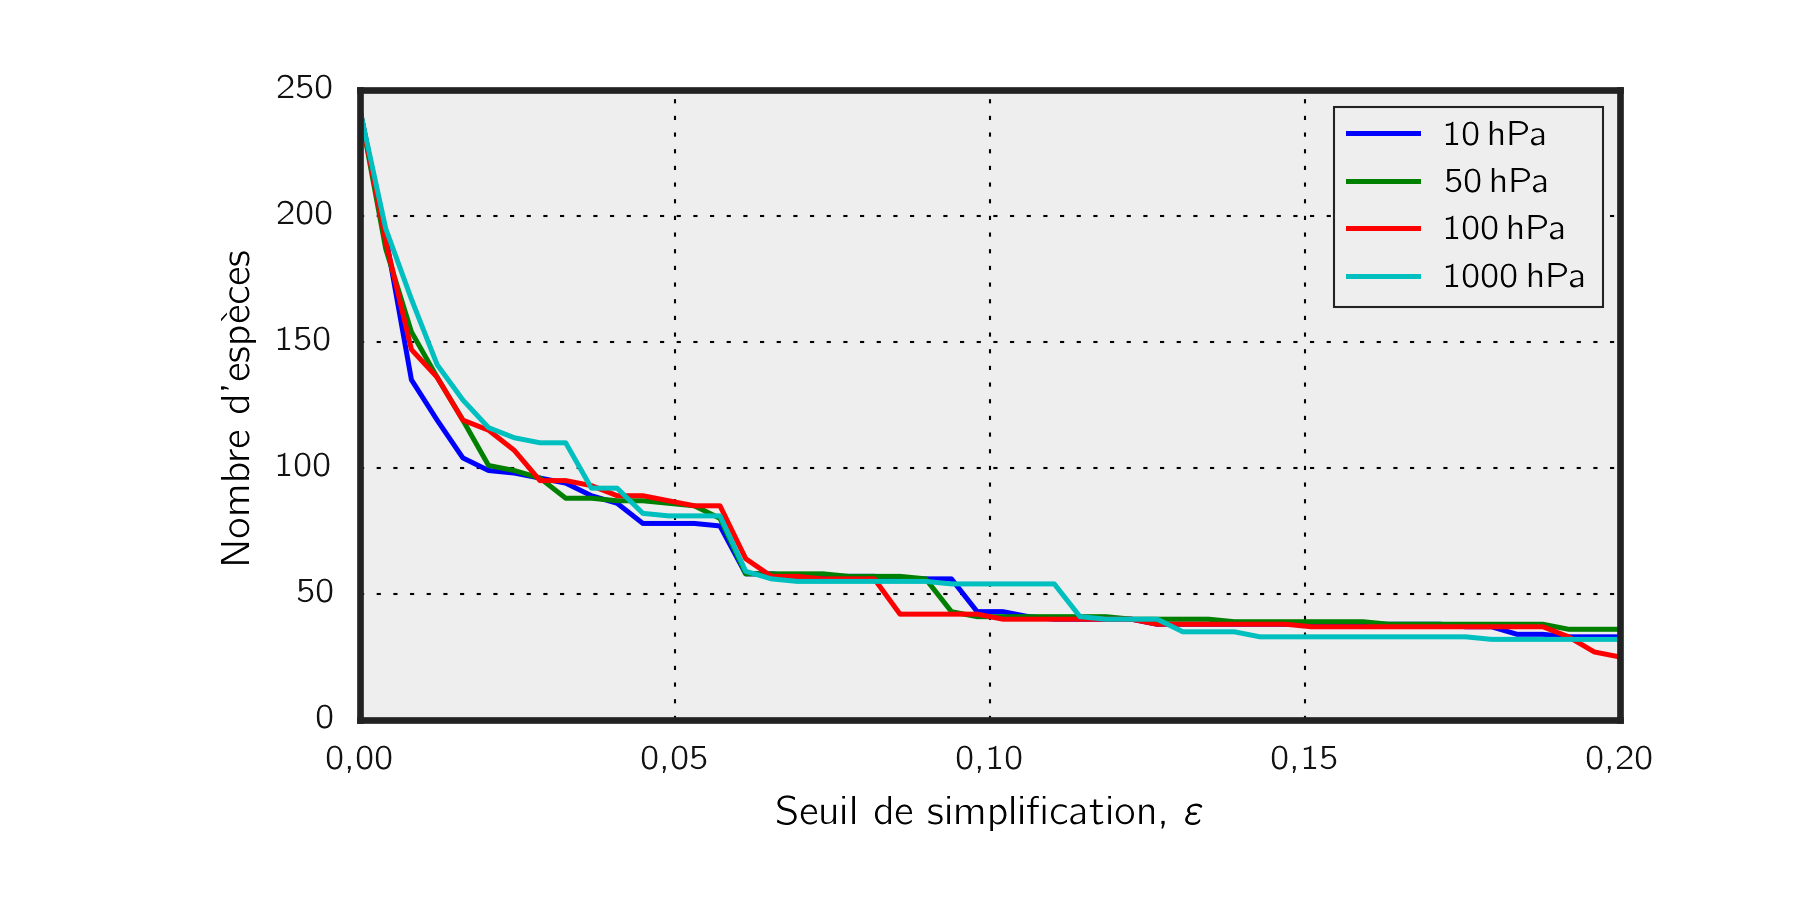
\includegraphics{figures/ch-05-kinetics-reduction-diagram}}
    
  \caption{\label{fig:diagramme_reduction}Diagramme du nombre d'espèces dans le mécanisme simplifié en fonction du seuil d'erreur $\varepsilon$ utilisé dans la simplification.}
\end{figure}

En ce qui concerne la représentativité des échantillons dans l'espace des états, la composition du Tableau~\ref{tab:atmosphere-starting} choisie comme point de départ représente la décomposition de l'acétylène pour des pressions partielles de \SIrange{3}{30}{\hecto\pascal}, dans la région d'intérêt pour la cémentation à partir des hydrocarbures et considère les impuretés typiques présentes dans les bouteilles de \ch{C2H2} dans une proportion qui est celle proposée par \citet{Norinaga2007}. Naturellement, cette composition n'est qu'un choix préliminaire à la simplification et on testera par la suite sa validité: les compositions de départ ne doivent pas forcement être celles que l'on désire simuler de manière simplifiée, mais elles doivent préférentiellement s'en approcher. Ces limites dans l'espace des états de la simplification réalisée sont fournies Tableau~\ref{tab:simplification-space}.

\begin{table}[h]
  \caption{\label{tab:simplification-space}Espace des états échantillonnés à partir de l'intégration isotherme pendant \SI{2}{\second} en réacteur parfaitement agité fermé de l'atmosphère fournie Tableau~\ref{tab:atmosphere-starting}. Un total de 10 échantillons de l'intégration du mécanisme de \citet{Norinaga2009} a été retenu entre les concentrations maximale et minimale en \ch{C2H2} pour la simplification du mécanisme.}
  
  \centering{}\footnotesize{}
  \begin{tabular}{\$c^c^c^c}
    \toprule[2pt]
    \rowstyle{\bfseries}
    Température                                         %1
    & \multicolumn{1}{c}{\bfseries{}Pression totale}    %2
    & \multicolumn{1}{c}{\bfseries{}Pression \ch{C2H2}} %3
    & \multicolumn{1}{c}{\bfseries{}Pression \ch{H2}}   %4
    \tabularnewline
    \midrule[2pt]
    \multirow{4}{2cm}[-9pt]{\centering{}\SI{1173}{\kelvin}} 
    & \SI{10}{\hecto\pascal}
    & \SIrange{2,7}{3,0}{\hecto\pascal}
    & \SIrange{0,0}{0,11}{\hecto\pascal}
    \tabularnewline[6pt]
    %
    & \SI{50}{\hecto\pascal}
    & \SIrange{11}{15}{\hecto\pascal}
    & \SIrange{0,0}{1,05}{\hecto\pascal}
    \tabularnewline[6pt]
    %
    & \SI{100}{\hecto\pascal}
    & \SIrange{17}{30}{\hecto\pascal}
    & \SIrange{0,0}{2,80}{\hecto\pascal}
    \tabularnewline[6pt]
    %
    & \SI{1000}{\hecto\pascal}
    & \SIrange{19}{30}{\hecto\pascal}
    & \SIrange{0,0}{3,70}{\hecto\pascal}
    \tabularnewline
    %
    \bottomrule
  \end{tabular}
\end{table}

Dans notre approche, composée des étapes d'échantillonnage, de balayage et de composition, le nombre d'espèces dans un mécanisme simplifié pour une valeur de $\varepsilon$ donnée Figure~\ref{fig:diagramme_reduction} est le résultat de l'union des mécanismes simplifiés obtenus sur tout l'espace des états échantillonnés pour une pression donnée: un mécanisme simplifié pour une combinaison $\varepsilon-P$ est le résultat de l'union de plusieurs mécanismes simplifiés, chacun obtenu pour un vecteur des états de l'échantillon de départ. Cela rend la simplification plus fiable et représentative de la région d'intérêt. La Figure~\ref{fig:diagramme_reduction} met en évidence un comportement de simplification presque indépendant de la pression: cela renforce l'hypothèse de faible dépendance des processus à trois corps sur la plage de pressions partielles étudiée. Cependant, cette affirmation est conditionnée à l'analyse de la séquence d'élimination des espèces dans les mécanismes obtenus:
\begin{enumerate}
  \item pour des valeurs de $\varepsilon{}<{}0,06$ les hydrocarbures de haut poids moléculaires sont éliminés dans un continuum indépendamment de la pression simulée; cela n'est pas forcement lié à l'absence de réactions décrivant ces espèces sitôt que le mécanisme complet comporte plus de 300 réactions pour les composés à plus de 7 atomes de carbone (C7+), mais aux faibles taux de réaction pour ces composés dans les échantillons utilisés;
  
  \item ce n'est qu'à $\varepsilon\ge{}0,06$ que les échelons de réduction du nombre d'espèces apparaissent et qu'il est possible d'éliminer des réactions liées principalement au naphtalène et au phénanthrène; ces éliminations sont pratiquement les mêmes pour toutes pressions utilisées;
  
  \item l'échelon suivant ($\varepsilon=0,08-0,11$) de réduction du nombre d'espèces est lié principalement aux hydrocarbures en C6; à partir de cette valeur, l'élimination du \ch{C2H4} et du \ch{C2H6} est aussi possible; comme le \ch{C2H4} est parmi les espèces majoritaires identifiées au Chapitre~\ref{ch:caracterisation_atmospheres}, il doit être inclus dans l'ensemble de départ pour ne pas être éliminé.
\end{enumerate}

Si l'on fait le suivi de la valeur $\varepsilon$ liée à l'élimination du \ch{C6H6}, on observe une décroissance de $\varepsilon=0,192$ à $\varepsilon=0,102$ en augmentant la pression partielle en \ch{C2H2} de \SIrange{3}{30}{\hecto\pascal} dans les gammes du Tableau~\ref{tab:atmosphere-starting}. En fixant $P(\ch{C2H2})=\SI{30}{\hecto\pascal}$, l'augmentation de la pression totale de \SIrange{100}{1000}{\hecto\pascal} n'a pas d'effet prononcé. La valeur de $\varepsilon$ associée à l'élimination du \ch{C6H6} monte à 0,118 \textemdash{} la pression totale ne joue pas un rôle essentiel sur l'importance du benzène dans cette plage de pressions. Cette espèce étant connue comme produit de polymérisation de l'acétylène~\cite{Norinaga2005}, son élimination à des valeurs plus faibles de $\varepsilon$ et à des pressions plus élevées est plutôt liée à sa transformation accélérée en HAP et donc à un caractère de composé intermédiaire rapide. Un effet inverse est observé pour les espèces liées à l'acétone: en augmentant la pression totale, leur importance augmente (élimination vers des valeurs plus élevées de $\varepsilon$) et donc leur influence dans l'initiation de la pyrolyse de l'acétylène devient plus importante~\cite{Norinaga2007}.

Cette discussion montre le genre de simplification possible à partir de la Figure~\ref{fig:diagramme_reduction} et des sous-mécanismes qui lui sont associés. La simplification des mécanismes selon la méthode de \citet{Lu2005} ne permet pas seulement la sélection des espèces fortement couplées au mécanisme dans son ensemble, mais fournit des pistes sur le type d'interaction entre certaines espèces. Pour la simulation des conditions expérimentales, on va conserver les mécanismes simplifiés à $\varepsilon=0,097$ pour intégrer le \ch{C6H6} dans toute la plage de pressions d'intérêt. Dans les conditions de simplification utilisées, il a été vérifié qu'une deuxième étape de simplification proposée par \citet{Lu2005} s'avère sans intérêt: essayer de simplifier ce mécanisme déjà simplifié n'apporte aucune élimination additionnelle d'espèces. Le Tableau~\ref{tab:reduced-mechanism} présente les 41 espèces à conserver dans ce mécanisme.% \textemdash{} les réactions avec d'autres espèces doivent être éliminées.
%Le mécanisme ainsi obtenu possède une matrice d'adjacence avec 41 n{\oe}uds (espèces), comptant le \ch{N2} qu'a été conservé comme porteur dans ce mécanisme, de densité 0,36 et donc de caractère moins creuse.

\begin{table}[!h]
  \caption{\label{tab:reduced-mechanism}Espèces à conserver dans le mécanisme simplifié de pyrolyse de l'acétylène dans des conditions représentatives de l'espace des états échantillonnés présenté Tableau~\ref{tab:simplification-space} pour le mécanisme de \citet{Norinaga2009}. Le mécanisme peut aussi prendre en compte \ch{N2} comme gaz porteur pour la source \ch{C2H2}. Pour les espèces qui ont une nomenclature differente de leur formule chimique dans le mécanisme de \citet{Norinaga2009}, leur notation dans le mécanisme est reprise entre parenthèses.}
  
  \centering{}\footnotesize{}%
  \begin{tabular}{p{3cm}lcp{3cm}l}
    \toprule[2pt]
    \multicolumn{5}{c}{Espèces dérivées à conserver}
    \tabularnewline
    \midrule[2pt]
    \ch{H2} & Dihydrogène  & & 
    \ch{H}  & Hydrogène        
    \tabularnewline[6pt]
    %
    \ch{CH4} & Méthane & & 
    \ch{CH3} & Méthyl       
    \tabularnewline[6pt]
    %
    \ch{C2H4} & Éthylène & & 
    \ch{C2H3} & Vinyl            
    \tabularnewline[6pt]
    %
    \ch{C2H6} & Éthane & & 
    \ch{C2H5} & Ethyl            
    \tabularnewline[6pt]
    %
    \ch{C4H2} & Diacétylène & & 
    \ch{C4H4} & Vinylacétylène   
    \tabularnewline[6pt]
    %
    \ch{C6H6} & Benzène & &
    \ch{C6H5} & Phényl           
    \tabularnewline[6pt]
    %
    \ch{C3H6} & Propène & & 
    \ch{C3H3} & Propargyl        
    \tabularnewline[6pt]
    %
    \ch{C3H5} (AC3H5) & Allyl & & 
    \ch{C3H4} (AC3H4) & Allène       
    \tabularnewline[6pt]
    %        
    \ch{C3H4} (PC3H4) & Propyne & & 
    \ch{C3H5} (SC3H5) & \chemfig{\Lewis{0.,}=-} 
    \tabularnewline[6pt]
    %
    \ch{C4H6} & 1,3-Butadiène & &
    \ch{C4H6} (C4H61) & 1-Butyne   
    \tabularnewline[6pt]
    %
    \ch{C4H6} (C4H612)  & 1,2-Butadine & &
    \multirow{2}{*}{\ch{C4H5} (I-C4H51)}   & \multirow{2}{*}{\chemfig{~-([:90]-[,0.1,,,,draw=none]\Lewis{0.,})-[:-30]}  }
    %\ch{C4H5} (I-C4H51) & \chemfig{~-([:90]-[,0.1,,,,draw=none]\Lewis{0.,})-[:-30]}  
    \tabularnewline[6pt]
    %
    \ch{C4H3} (I-C4H3)& \chemfig{~-([:90]-[,0.1,,,,draw=none]\Lewis{0.,})=} & &
    %- & - 
    \tabularnewline[6pt]
    %
    \ch{C5H6} & Cyclopentadiène & &
    \ch{C5H5} & Cyclopentadienyl 
    \tabularnewline[6pt]
    %
    \ch{C7H7} & Benzyl & & 
    \ch{C8H8} & 1,3,5,7-Cyclooctatétraène 
    \tabularnewline[6pt]
    %
    %
    \multirow{4}{3cm}[-6pt]{\ch{C9H8}}
    & \multirow{4}{3cm}[-6pt]{Indène} & &
    \multirow{4}{3cm}[-6pt]{\ch{C9H7}}
    & \multirow{4}{3cm}{\chemfig{[:60]*6(-*5(-=-\Lewis{0.,}-)=-=-=)}}
    \tabularnewline[6pt]
    & & & & 
    \tabularnewline[6pt]
    & & & &
    \tabularnewline[6pt]
    & & & &
    \tabularnewline[6pt]
    %    
    \ch{C8H6} (A1C2H)  & Phénylacétylène & &
    \ch{C8H8} (A1C2H3) & Styrène
    \tabularnewline[6pt]
    %
    \ch{C10H8} (A2) & Naphtalène & &
    \ch{CO}         & Monoxyde de carbone
    \tabularnewline[6pt]
    %
    \ch{C11H10} (A2CH3-2) & 2-Methylnaphthalène & &
    \ch{C11H9} (A2CH2-2)  & 2-Naphthylmethyl
    \tabularnewline[6pt]
    %
    \ch{CH3COCH3} & Acétone & & 
    \ch{CH3COCH2} & -              
    \tabularnewline[6pt]
    %
    \ch{CH2CO} & - & & 
    \ch{CH3CO} & -                
    \tabularnewline[6pt]
    %
    \bottomrule
  \end{tabular}
\end{table}

\section{Intégration des mécanismes cinétiques}
\label{sec:integration-mecanismes}

Les fondements des processus cinétiques chimiques selon la loi d'action de masse ont été introduits dans la Section~\ref{sec:cinetique}. Quelques modifications ont été discutées pour intégrer les processus dépendant de la pression et sur les parois. Ce paragraphe vise à comparer différents mécanismes cinétiques d'intérêt pour la carbonitruration à basse pression dans des conditions reproduisant les expériences réalisées et à comparer les résultats obtenus.

\subsection{Pyrolyse de l'acétylène}

Le mécanisme cinétique choisi pour la simulation de la pyrolyse de l'acétylène a été exploré de manière exhaustive dans la littérature~\cite{Norinaga2007,Norinaga2007ii,Khan2008,Norinaga2009}. Nous l'utilisons ici pour interpréter les expériences réalisées et utiliser les résultats produits pour réaliser une modélisation des étapes de cémentation à basse pression. On commence par une analyse globale de la pyrolyse du \ch{C2H2} puis on réalise l'intégration de la cinétique selon un modèle de réacteur piston, ce qui inclut le mécanisme simplifié du paragraphe précédent.

\subsubsection{Pyrolyse de l'acétylène: modèle global à pression atmosphérique}
\label{sec:simulation-acetylene-melange-pa}

En raison du faible nombre de Bodenstein ($Bo{}<{}10$) évalué dans nos conditions opératoires à la pression atmosphérique (Section~\ref{sec:dynamique_experimentale}), on utilise le modèle de mélange complet pour intégrer la conversion de l'acétylène. L'intégration de l'Équation~\ref{eq:maximum_mixedness_num} est faite directement sans prendre en compte les changements de volume associés à la pyrolyse du \ch{C2H2}. Cela n'est possible que pour les systèmes dilués, comme le mélange \ch{N2 - 0,02 C2H2}, pour lesquels de faibles variations entre les débits à l'entrée et à la sortie du réacteur sont observées à l'état stationnaire.

Le calcul de la vitesse globale de pyrolyse $\dot{\omega}_{i}$ est effectué en utilisant un modèle exponentiel d'ordre $n$ donné par $\dot{\omega}_{i}=-kc_{i}^{n}$. \citet{Norinaga2005} fournissent seulement les paramètres $k=1,5$ et $n=2,7$ pour la pyrolyse de l'acétylène à \SI{1173}{\kelvin} et à des pressions entre \SIlist{20;150}{\hecto\pascal}. Selon certains auteurs~\cite{Norinaga2005}, cet ordre $n=2,7$ est en bon accord avec la proposition de \og{}pyrolyse par polymérisation\fg{} en suivant le chemin de réaction \ch{C2H2 + C2H2 <=> C4H4} puis \ch{C2H2 + C4H4 <=> C6H6}, qui s'avère être le branchement principal~\cite{Norinaga2007} à l'origine de la décomposition du précurseur \ch{C2H2} dans la plage de températures étudiée. Ce chemin est responsable de la formation du benzène qui ensuite peut subir des réactions de condensation et induire formation d'hydrocarbures aromatiques polycycliques (HAP)~\cite{Ziegler2005a,Norinaga2009}. 

En utilisant des interpolations des courbes de distribution de temps de séjour expérimentales $E(t_{s})$ (Figure~\ref{fig:residence_time_distribution_raw}), la prédiction de la conversion peut être finalement réalisée à partir de l'intégration numérique de l'Équation~\ref{eq:maximum_mixedness_num}. Après des essais avec les paramètres proposés par \citet{Norinaga2005} ($k=1,5$ et $n=2,7$), nous avons montré que pour reproduire nos résultats expérimentaux à pression atmosphérique avec une excellente précision, on devait fixer $k=1,55$ et $n=2,85$: cela est raisonnable en fonction des temps de séjour beaucoup plus longs (et donc de pyrolyse dans un état beaucoup plus avancé) que ceux utilisés dans la dérivation des paramètres par \citet{Norinaga2005}. La valeur $n=2,85$ peut aussi indiquer une tendance \textendash{} associée au temps de séjour très long de l'ordre de \SI{200}{\second} \textendash{} plus favorable à la formation des HAP: une valeur $n=3$ correspond à la limite du processus global \ch{3 C2H2 <=> C6H6}, qui est à l'origine des composés lourds. 

Le Tableau~\ref{tab:maximum_mixedness_prediction} compare les mesures expérimentales aux prédictions réalisées à partir de la distribution de temps de séjour et du modèle global. Pour un débit de \SI{500}{\sccm} on obtient un bon accord entre les valeurs comparées \textemdash{} soit un écart de 4\% entre mesures et simulation si le réacteur n'est pas chargé d'un échantillon métallique. Pour les autres débits employés, l'écart entre mesures et simulation augmente mais l'ordre de grandeur de conversion du \ch{C2H2} reste bien représenté: à la sortie il ne reste qu'entre 1,5 et 2,4\% de l'acétylène introduit dans le réacteur non-chargé. Ces observations renforcent l'hypothèse d'une faible influence de la pression à partir de \SI{20}{\hecto\pascal} dans le mécanisme de \citet{Norinaga2009}, ce qui permet la simulation du procédé basse pression en utilisant de l'acétylène dilué à la pression atmosphérique. Les constantes $k$ et $n$ dérivées à basse pression permettent en effet de reproduire l'état d'avancement de la pyrolyse à la pression atmosphérique avec des pressions partielles en \ch{C2H2} à l'entrée de l'ordre de \SI{20}{\hecto\pascal}.

\begin{table}[h]
  \caption{\label{tab:maximum_mixedness_prediction}Comparaison entre les fractions molaires de \ch{C2H2} mesurées et prédites à la sortie du réacteur selon le modèle de mélange complet avec une loi cinétique $\dot{\omega}_{\ch{C2H2}}=1,55{}\times{}c_{\ch{C2H2}}^{2,85}$ et des distributions de temps de séjour correspondant aux conditions simulées \textemdash{} voir Chapitre~\ref{ch:caracterisation_atmospheres}.}
  
  \centering{}\footnotesize{}%
  \begin{tabular}{\$c^c^c^c^c^c}
    \toprule[2pt] 
    \rowstyle{\bfseries}
    \multirow{2}{*}[-3pt]{Chargement} &
    \multirow{2}{*}[-3pt]{Débit \sccm} &
    \multicolumn{3}{c}{\bfseries Fraction molaire -- \ch{C2H2}} &
    \multirow{2}{*}[-3pt]{Rapport}
    \tabularnewline
    \cmidrule{3-5}
    \rowstyle{\bfseries}
    & &
    Entrée $\times10^{2}$  &
    Mesurée $\times10^{3}$ & 
    Simulée $\times10^{3}$ & 
    \tabularnewline
    \midrule[2pt] 
    Non-chargé  & 250  & 2,0 & 3,67 & 3,10 & 0,85\tabularnewline[3pt]
    Non-chargé  & 500  & 2,0 & 4,25 & 4,36 & 1,04\tabularnewline[3pt]
    Non-chargé  & 1000 & 2,0 & 6,96 & 5,15 & 0,74\tabularnewline[3pt]
    Chargé      & 500  & 0,5 & 2,65 & 2,61 & 0,98\tabularnewline[3pt]
    Chargé      & 500  & 1,0 & 3,57 & 3,56 & 0,99\tabularnewline
    \bottomrule
  \end{tabular}
\end{table}

\subsubsection{Pyrolyse de l'acétylène: modèle global à basse pression}
\label{sec:simulation-acetylene-melange-bp}

Une fois vérifié le bon accord obtenu entre les expériences et les prédictions de conversion à pression atmosphérique, on s'intéresse à l'obtention d'une expression d'ordre global analogue pour nos mesures expérimentales sous pression réduite (Figure~\ref{fig:acetylene_bp}). Pour réaliser ce traitement de données, on considère une zone homogène de \SI{20}{\centi\metre} à la température de décomposition, ce qui est raisonnable vus les profils de la Figure~\ref{fig:temperature_profiles_bp}. L'approche de temps fractionnel (Équation~\ref{eq:fractional_time}) est employée dans les interpolations qui sont faites en utilisant une expression d'Arrhenius pour obtenir la dépendance de la constante cinétique avec la température. En l'absence de données de temps de séjour à basse pression, $\tau_{eff}$ est calculé en fonction du débit, de la température et de la pression, ce qui est possible en raison de la faible contraction en volume du gaz $\delta_{\dot{V}}$ lors de la pyrolyse \textemdash{} voir Section~\ref{sec:simulation-acetylene-piston}.

\begin{equation}
c_{i}^{1-n}-c_{i0}^{1-n}=k(T)(n-1)\tau_{eff}
\label{eq:fractional_time}
\end{equation}

Ce traitement de données est résumé Figure~\ref{fig:plug-flow-fit}, où l'on rassemble les fractions en \ch{C2H2} résiduel simulées (traits) comparées aux mesures expérimentales (points) pour les pressions de \SIlist{50;100}{\hecto\pascal}. Alors que les résultats sont rapportés séparément par pression et par débit, une seule interpolation de l'Équation~\ref{eq:fractional_time} a été réalisée pour tous les points expérimentaux. Les conditions de départ correspondent à un débit total de \SI{222}{\sccm} composé de \ch{N2 - 0,36 C2H2} (Tableau~\ref{tab:pyrolysis-conditions-bp}). Comme le temps de séjour $\tau_{eff}$ a été estimé à partir des conditions hydrodynamiques et de la température \textendash{} les autres paramètres du problème étant inchangés \textendash{} au moyen de l'Équation~\ref{eq:fractional_time}, nous avons choisi de rapporter les résultats Figure~\ref{fig:plug-flow-fit} en fonction de la température. Les courbes correspondent aux conversions calculées selon l'Équation~\ref{eq:fractional_time} en utilisant les paramètres du modèle global fournis Équation~\ref{eq:global-acetylene}. Il n'a pas été possible d'intégrer les mesures réalisées à \SI{30}{\hecto\pascal} dans ce modèle du fait de l'erreur importante qu'elles introduisent: une forte oscillation de pression a lieu pendant le prélèvement de l'échantillon de gaz, ce qui affecte la mesure de manière non--négligeable. Comme cela a été mentionné Chapitre~\ref{ch:caracterisation_atmospheres}, cette pression représente la limite minimale pour l'acquisition de chromatogrammes et les mesures sont moins reproductibles, ce qui n'est pas le cas à \SI{100}{\hecto\pascal}. 

\begin{equation}
\dot{\omega}_{\ch{C2H2}}={3,86\times{}10^4}
\exp\biggr(\frac{-\SI{100,7}{\kilo\joule}}{RT}\biggr)c_{\ch{C2H2}}^{2,163}{}\times{}10^{-6}\si{\mole\per\cubic\centi\metre\per\second}
\label{eq:global-acetylene}
\end{equation}

\begin{figure}[h]
  \centering\resizebox{0.98\textwidth}{!}{%
    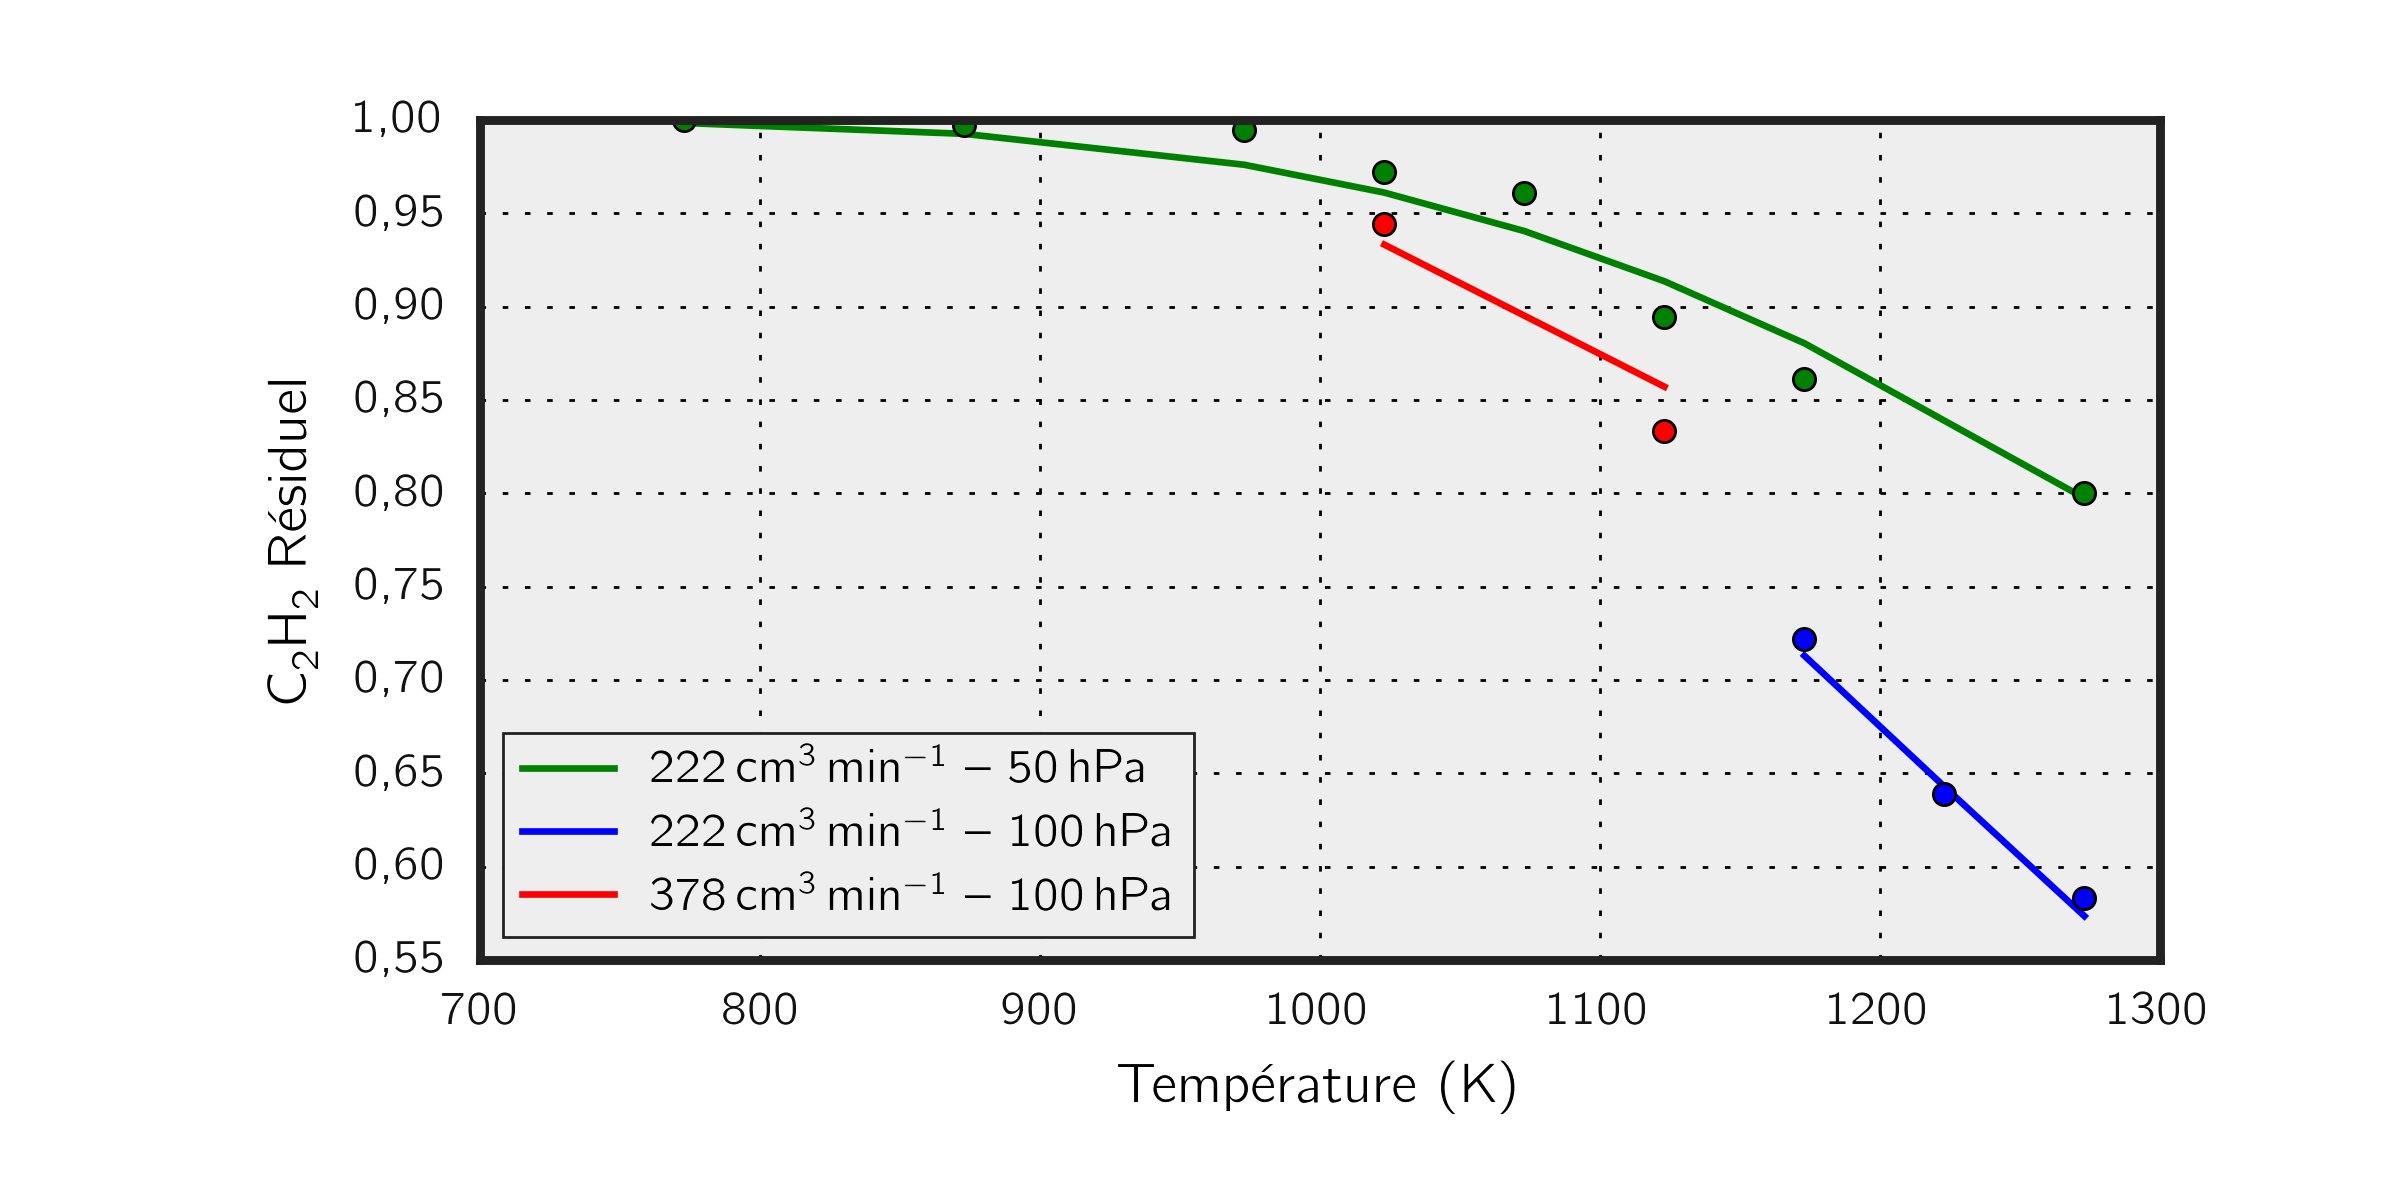
\includegraphics{figures/ch-05-kinetics-plug-flow-fit}}
    
  \caption{\label{fig:plug-flow-fit}Fraction d'acétylène résiduelle en fonction de la température. Modèle global de temps fractionnel. Comparaison entre les valeurs simulées et les données de la Section~\ref{sec:pyrolyse_acetylene_bp}.}
\end{figure}

La dérivation de l'Équation~\ref{eq:global-acetylene} à partir des données expérimentales conduit à des énergies d'activation comprises entre \SIlist{85;115}{\kilo\joule\per\mole} si l'on utilise séparément les données à \SIlist{50;100}{\hecto\pascal}, respectivement. Si l'on considère tous les points présentés sur la Figure~\ref{fig:plug-flow-fit}, une valeur proche de \SI{100}{\kilo\joule\per\mole} est obtenue. Cette valeur est inférieure à celles des réactions de condensation \ch{C2H2 + C2H2 <=> C4H4} et \ch{C2H2 + C4H4 <=> C6H6} rapportées dans le mécanisme de \citet{Norinaga2009} \textendash{} entre \SIlist{126;179}{\kilo\joule\per\mole} \textendash{} et donc cette valeur est raisonnable si l'on tient compte des étapes intermédiaires de plus faible activation. À \SI{1173}{\kelvin}, on calcule une constante $k=1,26$, inférieure à $k=1,5$ rapportée par \citet{Norinaga2005}. Les données conduisent à un ordre global $n=2,16$, aussi inférieur à celui rapporté dans la littérature~\cite{Norinaga2005}. Cette valeur est encore en accord avec la séquence de décomposition proposée~\cite{Norinaga2005,Becker1998177} mais est moins favorable à la formation de \ch{C6H6}. La précision des données et le manque de mesures pour le benzène ne permettent pas une discussion plus approfondie de ce comportement. De plus, la dilution dans l'azote comme gaz porteur peut jouer un rôle qui n'a pas été mis en évidence dans cette étude. Le Tableau~\ref{tab:constantes-globales} compare les modèles globaux utilisés de décomposition de l'acétylène.

\begin{table}[h]
  \caption{\label{tab:constantes-globales}Comparaison entre les paramètres de vitesse de décomposition de l'acétylène proposés par \citet{Norinaga2005} et dérivés de cette étude. Vitesse globale de décomposition $\dot{\omega}_{\ch{C2H2}}$ donnée en \si{\mole\per\cubic\centi\metre\per\second}.}
  
  \resizebox{\textwidth}{!}{
  \centering{}\footnotesize{}
  \begin{tabular}{\$l^c^c^c^l}
    \toprule[2pt]
    \rowstyle{\bfseries}
    Source 
    & Mélange 
    & Température 
    & Pression 
    & Vitesse globale $\dot{\omega}_{\ch{C2H2}}$
    \tabularnewline
    \midrule[2pt]
    \citet{Norinaga2005}
    & \ch{C2H2}
    & \SI{1173}{\kelvin}
    & \SIrange{20}{150}{\hecto\pascal}
    & $1,500{}\times{}c_{\ch{C2H2}}^{2,700}$
    \tabularnewline[9pt]
    \multirow{2}{3cm}[-3pt]{Cette étude}
    & \ch{N2 - 0,02 C2H2}
    & \SI{1173}{\kelvin}
    & \SI{1000}{\hecto\pascal}
    & $1,550{}\times{}c_{\ch{C2H2}}^{2,850}$
    \tabularnewline[9pt]
    & \ch{N2 - 0,36 C2H2}
    & \SIrange{773}{1273}{\kelvin}
    & \SIrange{50}{100}{\hecto\pascal}
    & $3,86{}\times{}10^{-2}{}\exp(\nicefrac{-12111}{T}){}c_{\ch{C2H2}}^{2,163}$
    \tabularnewline
    \bottomrule
  \end{tabular}
  }
\end{table}

Du point de vue pratique, les paramètres cinétiques de l'Équation~\ref{eq:global-acetylene} peuvent être utilisés pour estimer le flux d'acétylène arrivant aux pièces dans une installation industrielle. Cela peut être fait dans un premier temps en considérant la vitesse calculée du gaz injecté et la distance linéaire du point d'injection aux pièces. Il faut tenir compte que notre estimation de ces paramètres a été perturbée par le gradient de température du réacteur \textendash{} on a fait l'hypothèse qu'aucune décomposition importante n'a lieu avant ou après la zone des gradients en température du réacteur \textendash{} et aussi par le fait que nous n'avons pas mesuré le débit en sortie pour prendre en compte des effets de changement de volume du mélange injecté sur le temps de séjour. Dans le cas des expériences de \citet{Norinaga2005}, les paramètres ont été dérivés à partir d'expériences réalisées proches du cas idéal isotherme et avec des temps de séjour généralement plus courts que les nôtres. De cette manière, on suppose que les résultats de la littérature~\cite{Norinaga2005} représentent la limite supérieure de conversion, alors que notre loi globale représente le seuil inférieur. Une comparaison entre ces modèles est fournie Figure~\ref{fig:conversion-low-pressure}. Dans ce cas, notre principale contribution est l'inclusion de l'effet de la température sur la pyrolyse globale, comme cela est montré Figure~\ref{fig:conversion-temperature-effect}.

\subsubsection{\label{sec:simulation-acetylene-piston}Pyrolyse de l'acétylène: réacteur piston}

La section précédente ayant traité des processus globaux, on s'intéresse maintenant à l'intégration de la cinétique détaillée de pyrolyse de \ch{C2H2} à basse pression avec le mécanisme de \citet{Norinaga2009}. Notre objectif est aussi de valider le mécanisme simplifié obtenu à la Section~\ref{sec:simplification-mechanisme}. L'écoulement étant laminaire avec un nombre de Reynolds de l'ordre de l'unité et des vitesses importantes produites par l'écoulement à basse pression, les expériences réalisées en dessous de \SI{100}{\hecto\pascal} sont simulées en utilisant un modèle de réacteur de type piston avec le profil mesuré de températures imposé sur les parois du tube (Figure~\ref{fig:temperature_profiles_bp}). En raison de l'asymétrie de ces profils, l'Équation~\ref{eq:wall-temperature} a été utilisée pour imposer la température $T_{p}(x)$ sur les parois à une distance $x$ de l'entrée de la zone chauffée. Les températures $T_{a}$, $T_{c}$ et $T_{s}$ désignent les températures ambiante, de contrôle dans la zone chaude et à la sortie du réacteur, respectivement. Les paramètres $x_{1-2}$ et $m_{1-2}$ ont été ajustés aux données expérimentales pour permettre d'imposer cette condition aux limites dans les simulations.

\begin{figure}[!h]
	\centering
	\subfloat[\label{fig:conversion-low-pressure}Comparaison entre les modèles.]{
		\centering\resizebox{0.98\textwidth}{!}{%
			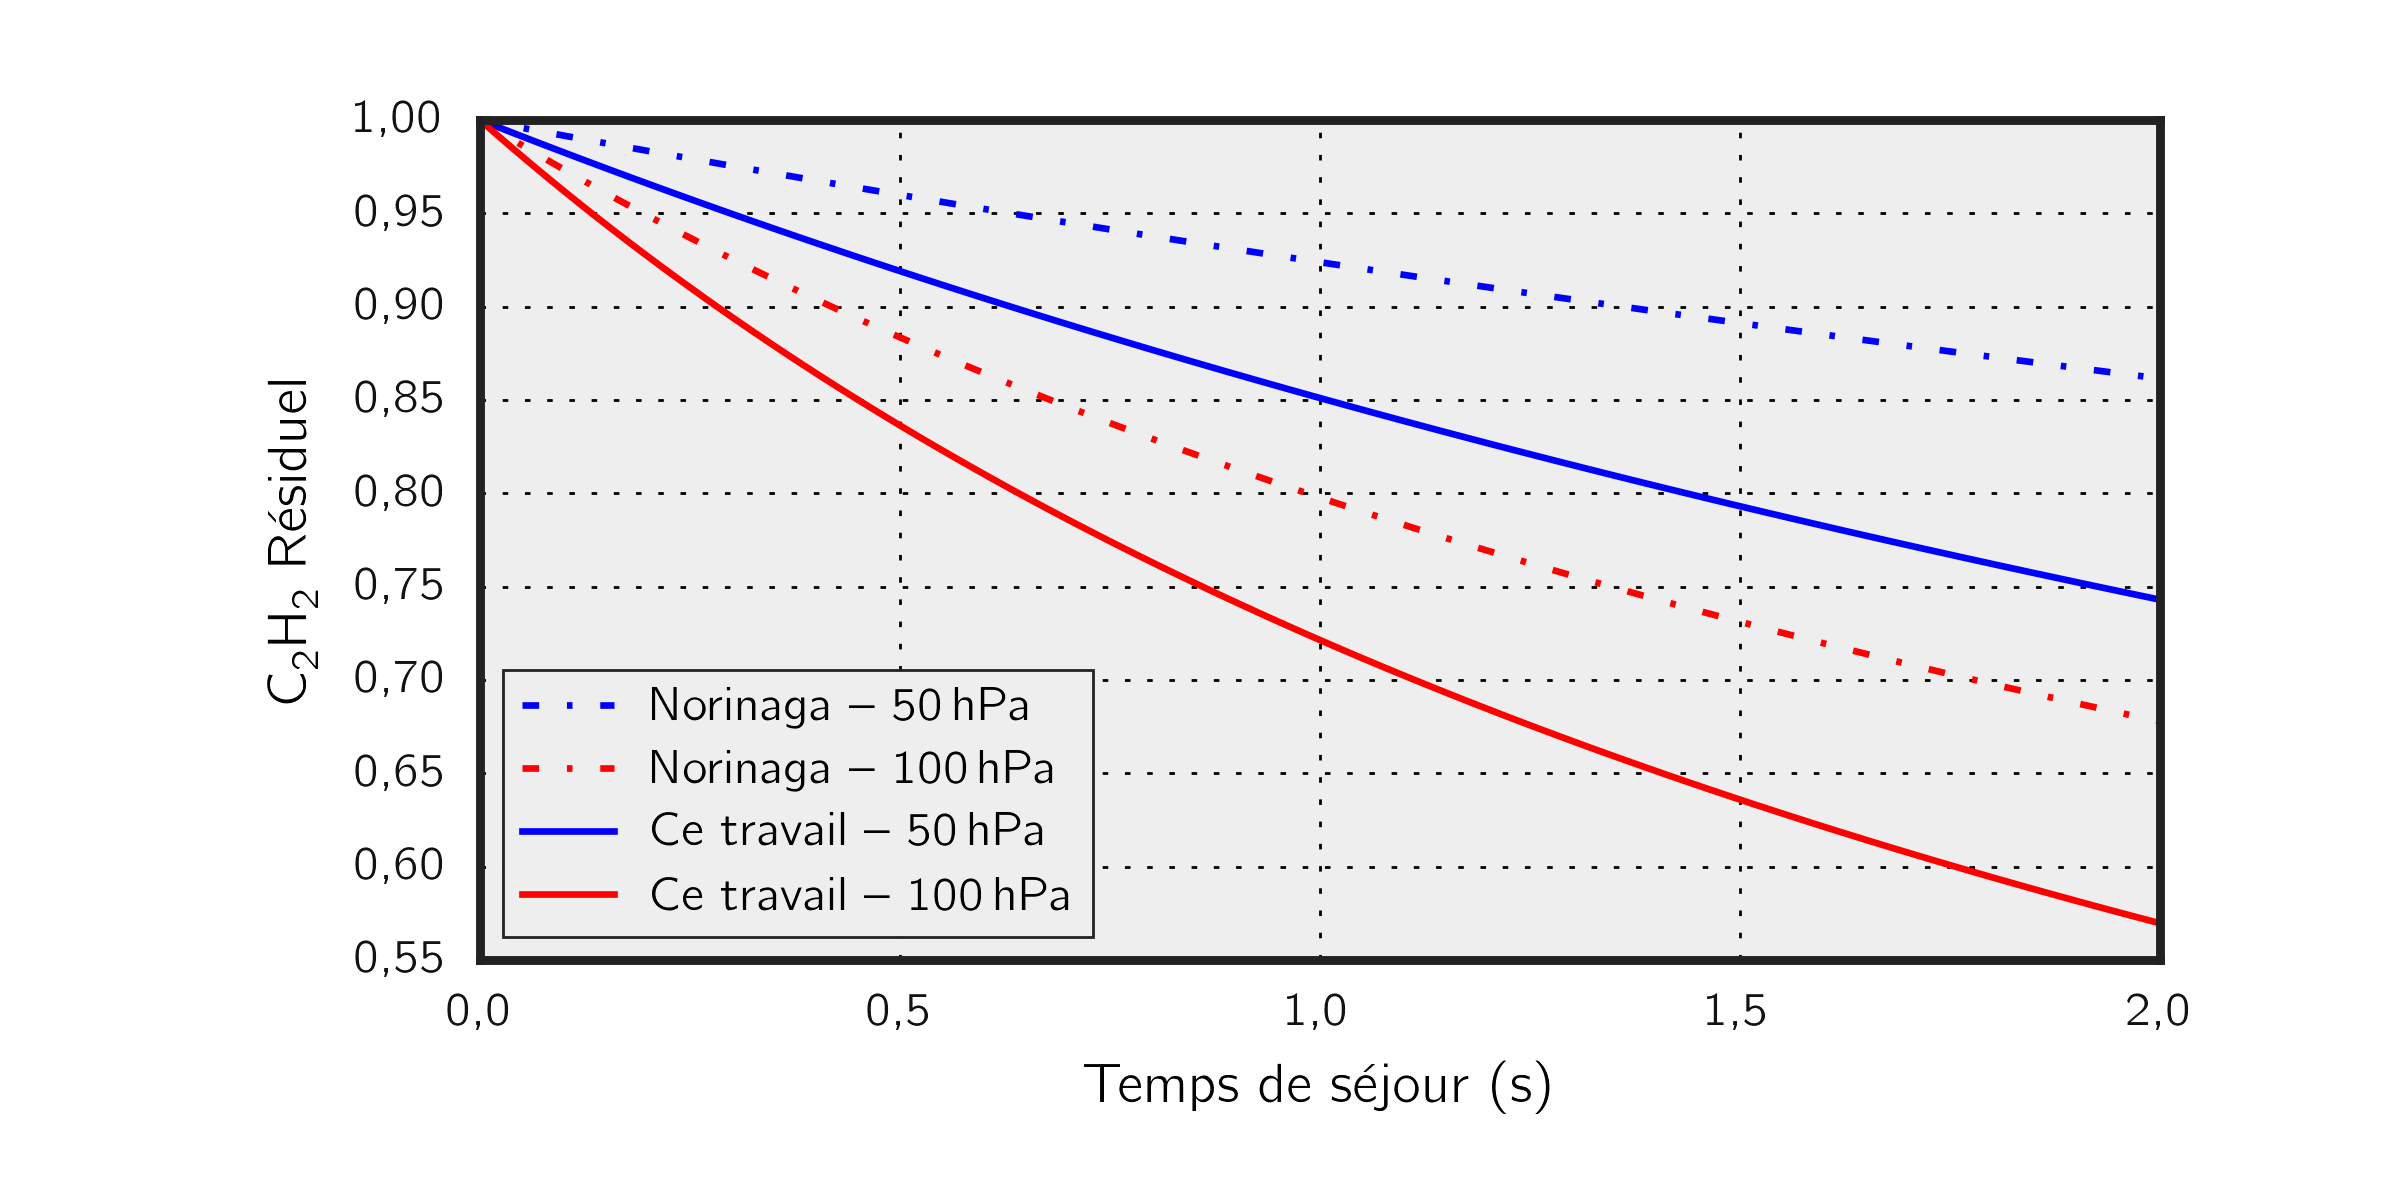
\includegraphics{figures/ch-05-kinetics-conversion-low-pressure}}
	}\\
	\subfloat[\label{fig:conversion-temperature-effect}Effet de la température sur la conversion.]{
		\centering\resizebox{0.98\textwidth}{!}{%
			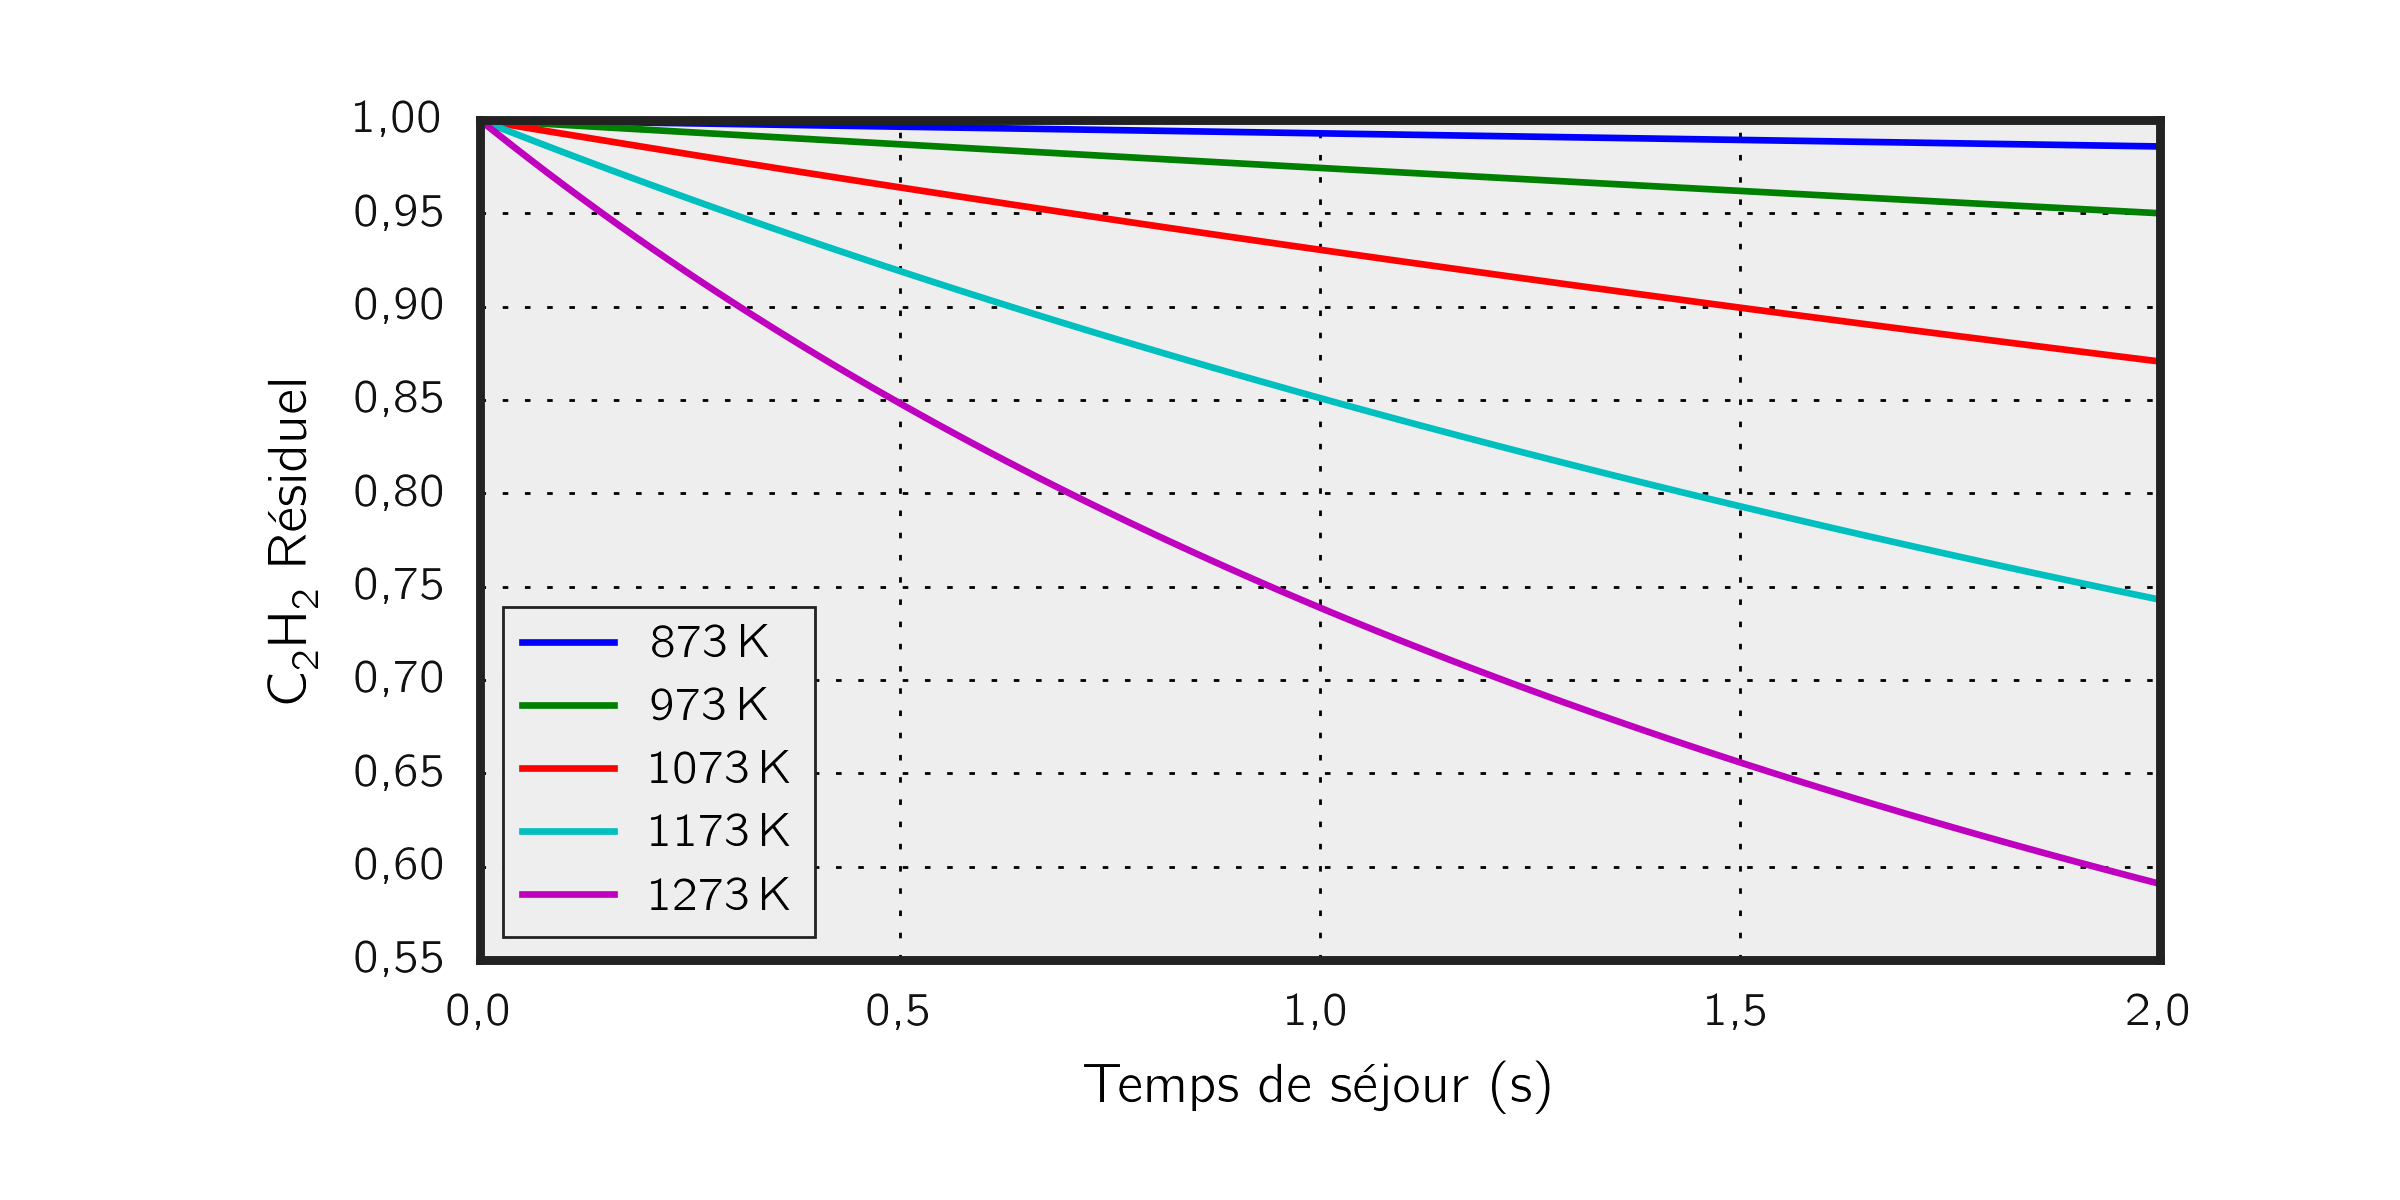
\includegraphics{figures/ch-05-kinetics-conversion-temperature-effect}}
	}
	
	\caption{Modèle global de décomposition de \ch{C2H2}: \protect\subref{fig:conversion-low-pressure} comparaison entre l'expression globale de pyrolyse de l'acétylène obtenue par \citet{Norinaga2005} et celle dérivée dans cette section, \protect\subref{fig:conversion-temperature-effect} rôle de la température sur la conversion pour une atmosphère \ch{N2 - 0,36 C2H2} à \SI{50}{\hecto\pascal} en termes de temps de séjour.}
\end{figure}

\begin{equation}
  T_{p}(x)=T_{a}+
  (T_{c}-T_{a}){}\biggr[1-\exp\biggr(-\frac{x}{x_{1}}^{m_{1}}\biggr)\biggr]-
  (T_{c}-T_{s}){}\biggr[1-\exp\biggr(-\frac{x}{x_{2}}^{m_{2}}\biggr)\biggr]
  \label{eq:wall-temperature}
\end{equation}

La bibliothèque de fonctions Cantera~\cite{Cantera2014} ne permet pas encore une implémentation d'un tel modèle de réacteur de type piston \textendash{} soit l'intégration d'un système d'équations différentielles algébriques, comprenant les équations de conservation des espèces et de l'énergie avec la contrainte $\rho{}u=\text{constant}$ \textendash{} et sa définition a donc été nécessaire. On peut regarder un réacteur de type piston comme une série de réacteurs parfaitement agités de volume infinitésimal $\mathrm{d}V=\pi{}r^{2}\mathrm{d}l$ à l'état stationnaire. La simulation du comportement \og{}piston\fg{} se fait donc en discrétisant l'axe du réacteur tubulaire en tranches de longueur $\mathrm{d}l$, chacune intégrée comme un réacteur parfaitement agité en utilisant l'état stationnaire de la tranche précédente comme composition à l'entrée. Un débit massique correspondant à la condition expérimentale est fixé à l'entrée de la première tranche dont la composition et la température évoluent dans le temps jusqu'à l'état stationnaire. Cette condition simulée est donc utilisée comme donnée d'entrée pour la deuxième tranche du réacteur et cela continue de proche en proche jusqu'à la sortie de la zone chaude. Ces simulations sont réalisées pour la pyrolyse en l'absence d'un échantillon métallique. Le flux massique est donc conservé tout au long du réacteur. 

\begin{figure}[!hb]
	\centering\resizebox{0.95\textwidth}{!}{%
		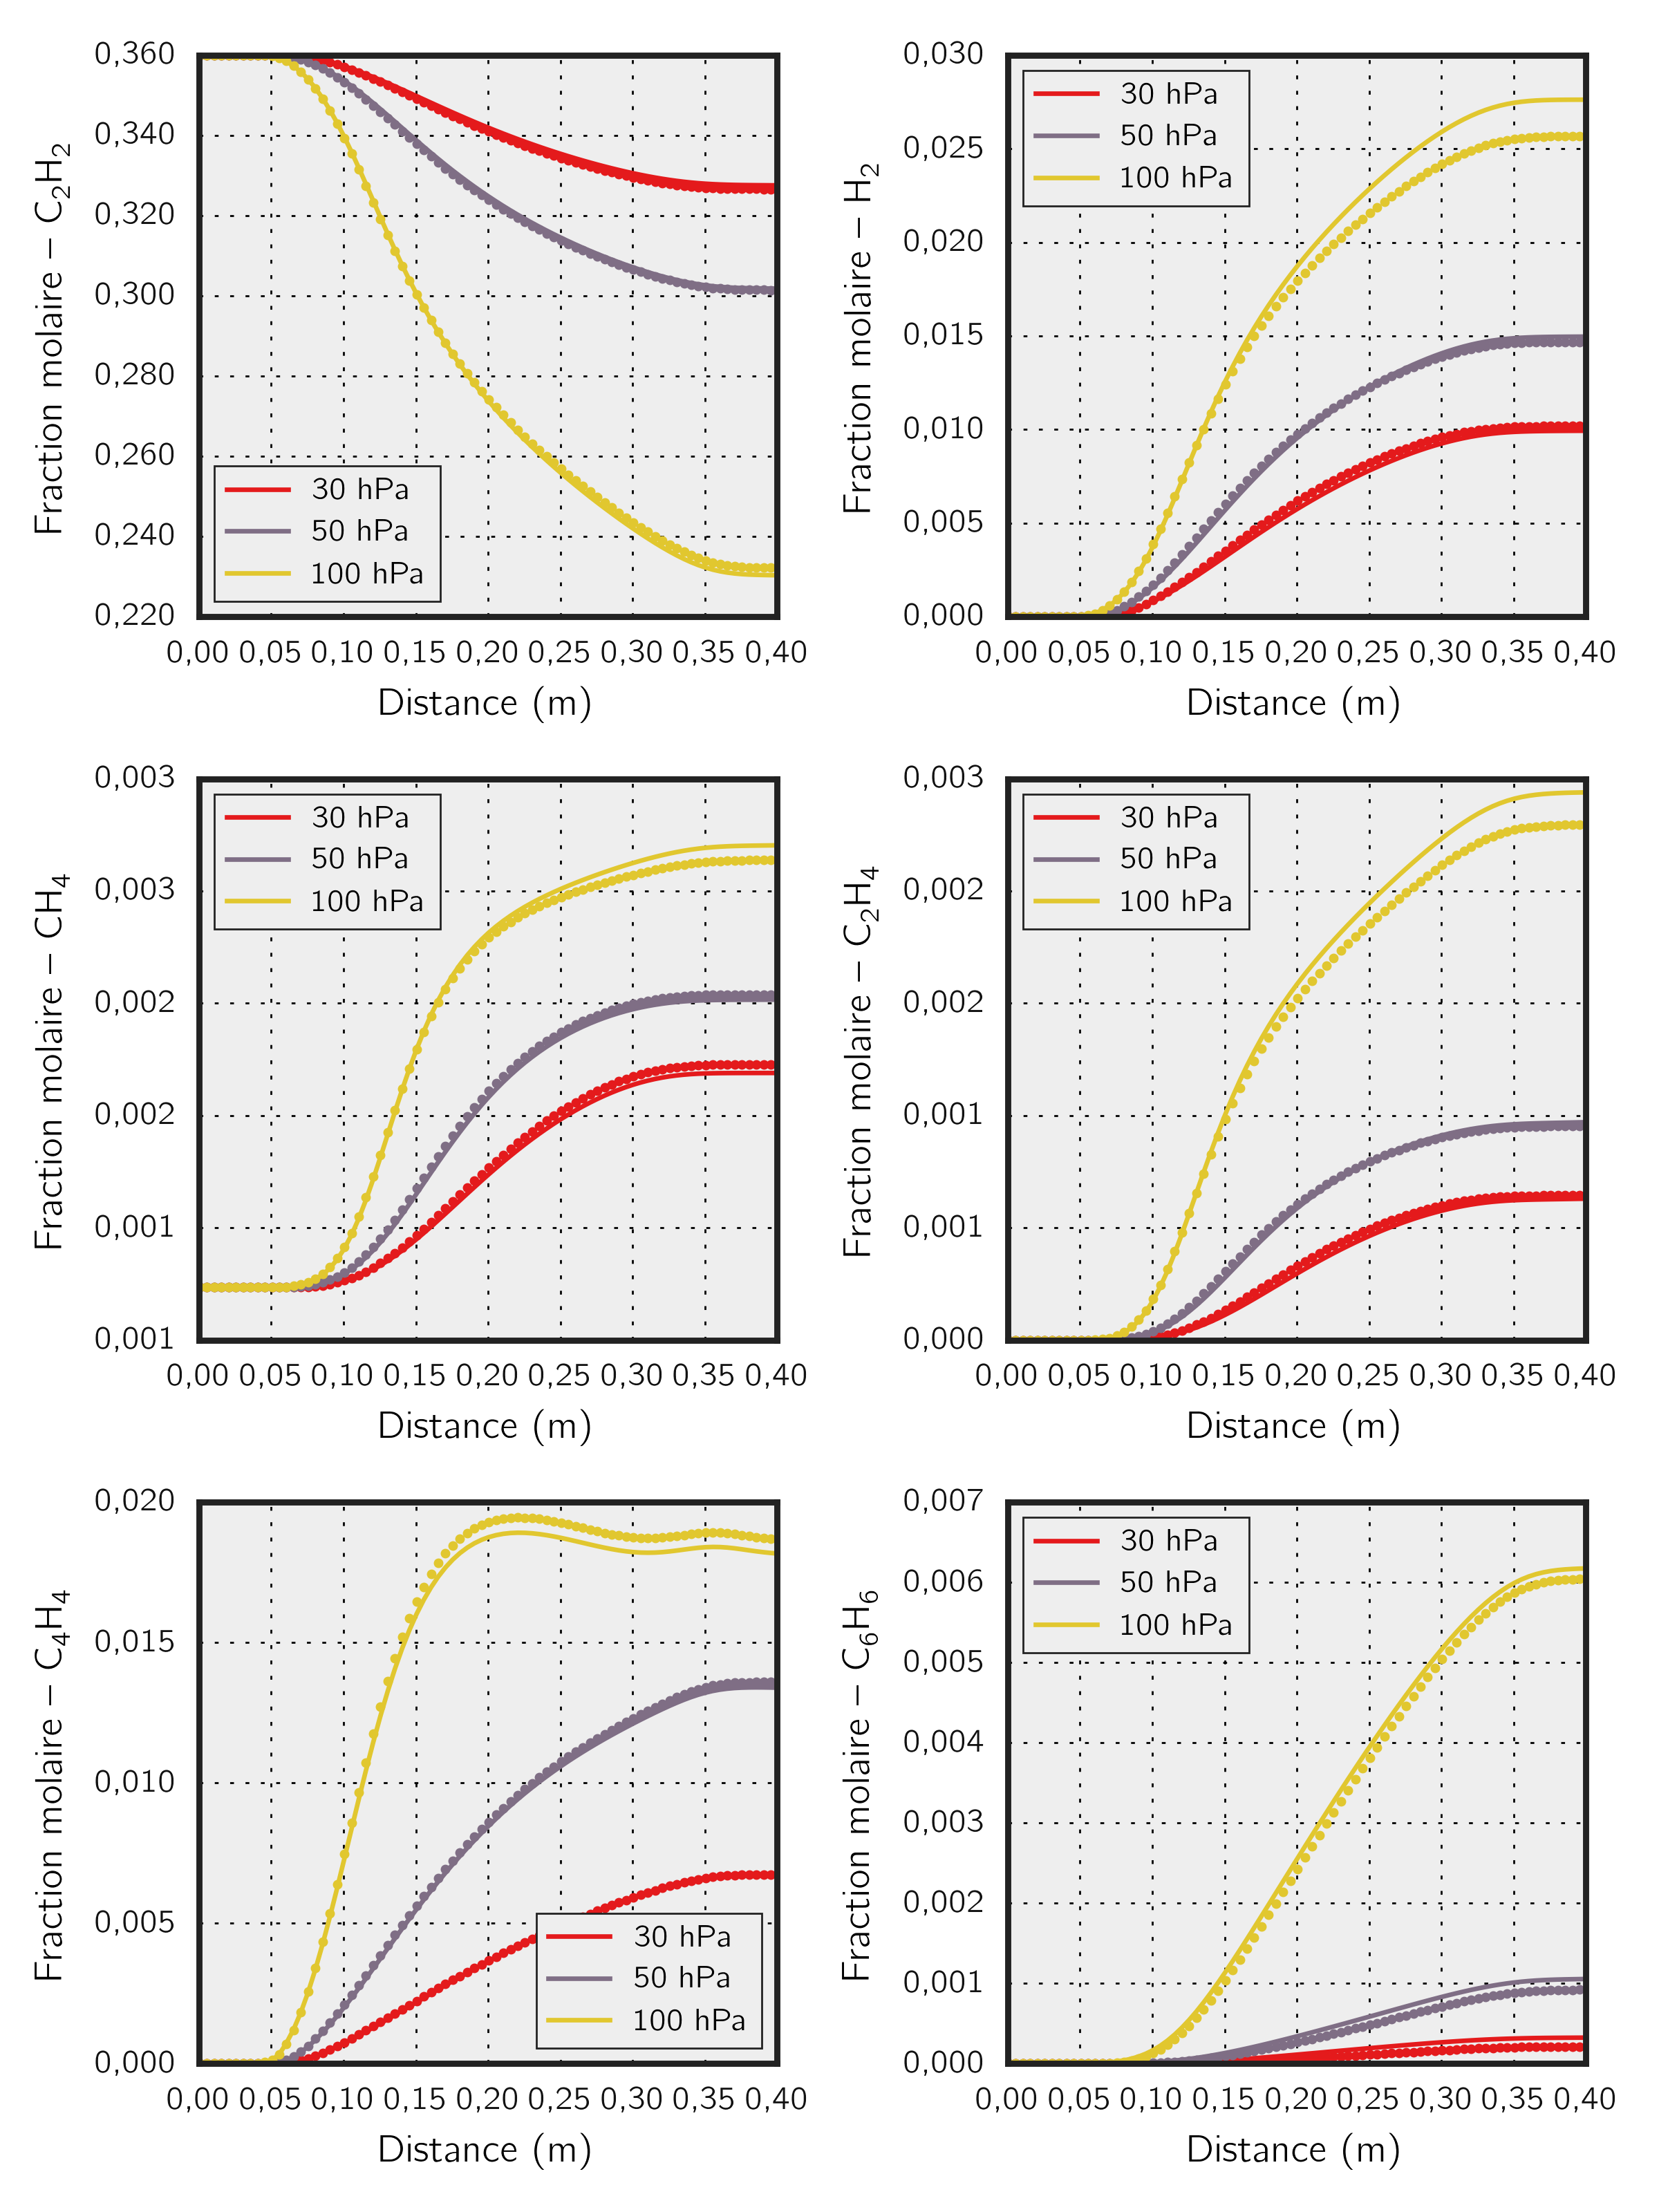
\includegraphics{figures/ch-05-kinetics-norinaga-simplification-1173K}}
	
	\caption{\label{norinaga-comparison-simplification-1173K}Comparaison entre des intégrations du mécanisme simplifié (points) et le mécanisme de \citet{Norinaga2009} (traits) de pyrolyse de l'acétylène dans réacteur de type piston avec palier de température à \SI{1173}{\kelvin}.}
\end{figure}

On trouve Figure~\ref{norinaga-comparison-simplification-1173K} l'intégration du mécanisme de \citet{Norinaga2009} en fonction de la position dans la direction de l'axe du réacteur pour les principaux hydrocarbures légers \textendash{} jusqu'à \ch{C6} \textendash{} et pour le \ch{H2}. Ces simulations sont simultanément comparées au mécanisme squelette obtenu Section~\ref{sec:simplification-mechanisme}. On observe l'effet de la pression sur la décomposition de \ch{C2H2} avec une formation importante de \ch{H2}, qui est le produit principal. Pour des pressions inférieures à \SI{50}{\hecto\pascal}, \ch{CH4} est d'avantage produit par rapport à \ch{C2H4}. Ce comportement est inversé à \SI{100}{\hecto\pascal}, pression à partir de laquelle on prédit des fractions plus importantes de \ch{C2H4}. En termes de position dans le réacteur, on vérifie une formation de \ch{C4H4} avant celle de \ch{C6H6} comme attendu en raison du chemin global décrit section précédente. 

Le mécanisme de \citet{Norinaga2009} a été simplifié à partir des simulations réalisées sans résoudre l'équation de l'énergie à \SI{1173}{\kelvin}. Cependant la simplification a été réalisée à cette température fixe, le mécanisme simplifié obtenu s'avère capable de reproduire \textendash{} Figure~\ref{fig:temperature_profiles_bp} \textendash{} les courbes obtenues à partir de l'intégration du mécanisme complet même dans les régions de gradient thermique du réacteur. À \SI{100}{\hecto\pascal} de pression totale, correspondant à \SI{36}{\hecto\pascal} de \ch{C2H2} dans nos expériences et simulations, le mécanisme simplifié commence à s'éloigner de la solution du mécanisme complet. Comme cette condition ne représente pas d'intérêt pour la cémentation, réalisée normalement en--dessous de \SI{20}{\hecto\pascal}, cet écart ne limite pas l'utilisation du mécanisme simplifié dans la simulation de la cémentation.
%~\footnote{Cela pourrait être contourné en réalisant une simplification dans un espace des états de pressions plus élevées, par exemple.}. 
L'Annexe~\ref{an:simplification-norinaga} présente des informations complémentaires des espèces plus lourdes du mécanisme simplifié et de son utilisation en dehors de l'espace des états de la simplification.

Le Tableau~\ref{tab:simulation_pfr_acetylene} compare les fractions molaires de l'acétylène mesurées en sortie du réacteur (Section \ref{sec:pyrolyse_acetylene_bp}) à celles prédites en utilisant le modèle de réacteur piston avec le mécanisme détaillé~\cite{Norinaga2009} et le mécanisme simplifié obtenu Section~\ref{sec:simplification-mechanisme}. Le débit $Q$ Tableau~\ref{tab:simulation_pfr_acetylene} est fourni à la pression atmosphérique à titre comparatif. Pour être précis, le débit massique devrait être employé, mais il est peu utile pour les expériences où l'on préfère utiliser le débit volumique. La pression est donnée sous forme d'une pression totale et l'atmosphère à l'entrée est composée d'un mélange \ch{N2 - 0,36 C2H2}. Pour déterminer la valeur de $\mathrm{d}l$ optimale, on commence avec $\mathrm{d}l=\SI{5}{\milli\metre}$ pour une première intégration. Ensuite, on réduit progressivement l'épaisseur des tranches de \SI{0,5}{\milli\metre} jusqu'au moment o\`{u} la différence relative des fractions molaires entre deux intégrations réalisées avec des $\mathrm{d}l$ consécutifs est inférieure à $10^{-6}$ pour chaque espèce. On trouve que la valeur $\mathrm{d}l=\SI{1}{\milli\metre}$ satisfaisait aux 14 conditions testées.

\begin{table}[h]
  \caption{\label{tab:simulation_pfr_acetylene}Simulations des fractions molaires en acétylène à la sortie du réacteur comparées aux mesures expérimentales. Atmosphère de départ composée de \ch{N2 - 0,36 C2H2}.}
  
  \centering{}\footnotesize{}%
  \begin{tabular}{\$c^c^c^c^c^c^c^c^c^c^c^c}
    \toprule[2pt]
    \rowstyle{\bfseries}
    \multirow{3}{*}[-3pt]{N} &
    {P} &
    {Q} &
    {T} &
    {$\tau_{\mathbf{eff}}$} &
    {$\delta_{\mathbf{\dot{V}}}$} &
    \multicolumn{5}{c}{\bfseries Fraction molaire en \ch{C2H2}}
    \tabularnewline
    \cmidrule{7-12}
    & 
    \multirow{2}{*}[+1pt]{\si{\hecto\pascal}}   &
    \multirow{2}{*}[+1pt]{\si{\sccm}}           & 
    \multirow{2}{*}[+1pt]{\si{\kelvin}}         & 
    \multirow{2}{*}[+1pt]{\si{\second}}         &
    \multirow{2}{*}[+1pt]{\%}                   & 
    \multicolumn{2}{c}{Mesures}              &
    \multicolumn{2}{c}{Mécanisme~\cite{Norinaga2009}} &
    \multicolumn{2}{c}{Simplifié}
    \tabularnewline
    \multicolumn{6}{c}{} & Valeur & $F-\%$ & Valeur & $\varepsilon-\%$ & Valeur & $\varepsilon-\%$
    \tabularnewline
    \midrule[2pt]
    %                                                   241            41                             35   
    1  &  50 & 222 &  773 & 1,836 & 0,0 & 0,352 & 97  & 0,360 & +2,3 & 0,360 & +2,3  \tabularnewline[3pt] % 0,360
    2  &  50 & 222 &  873 & 1,593 & 0,0 & 0,364 & 100 & 0,359 & -1,4 & 0,360 & -1,1 \tabularnewline[3pt] % 0,359
    3  &  50 & 222 &  973 & 1,417 & 0,2 & 0,364 & 100 & 0,356 & -2,2 & 0,356 & -2,2 \tabularnewline[3pt] % 0,355
    4  &  50 & 222 & 1073 & 1,278 & 0,8 & 0,346 & 95  & 0,340 & -1,7 & 0,340 & -1,7 \tabularnewline[3pt] % 0,339
    5  &  50 & 222 & 1123 & 1,236 & 1,5 & 0,312 & 86  & 0,321 & +2,9 & 0,321 & +2,9  \tabularnewline[3pt] % 0,319
    6  &  50 & 222 & 1173 & 1,197 & 2,2 & 0,307 & 84  & 0,302 & -1,6 & 0,301 & -2,0 \tabularnewline[3pt] % 0,295
    7  &  50 & 222 & 1273 & 1,140 & 1,6 & 0,288 & 79  & 0,287 & -0,3 & 0,288 & -0,0 \tabularnewline[3pt] % 0,286
    8  &  30 & 222 & 1173 & 0,713 & 0,9 & 0,323 & 89  & 0,327 & +1,2 & 0,327 & +1,2  \tabularnewline[3pt] % 0,323
    9  &  30 & 222 & 1223 & 0,696 & 1,0 & 0,314 & 86  & 0,320 & +1,9 & 0,319 & +1,6  \tabularnewline[3pt] % 0,324
    10 & 100 & 222 & 1173 & 2,443 & 6,3 & 0,249 & 68  & 0,230 & -7,6 & 0,232 & -6,8 \tabularnewline[3pt] % 0,235
    11 & 100 & 222 & 1223 & 2,363 & 6,0 & 0,226 & 62  & 0,219 & -3,1 & 0,221 & -2,2 \tabularnewline[3pt] % 0,231
    12 & 100 & 222 & 1273 & 2,294 & 4,9 & 0,201 & 55  & 0,208 & +3,5 & 0,212 & +5,5  \tabularnewline[3pt] % 0,222
    13 & 100 & 378 & 1023 & 1,556 & 0,9 & 0,343 & 94  & 0,342 & -0,3 & 0,342 & -0,3 \tabularnewline[3pt] % 0,340
    14 & 100 & 378 & 1123 & 1,443 & 3,2 & 0,298 & 82  & 0,292 & -2,0 & 0,288 & -3,4
    \tabularnewline % 0,285
    %4  &  50 & 222 & 1023 & & 0,35 & & \tabularnewline %REDO
    %9  &  30 & 222 & 1123 & 0,738 & 0,31 & 0,341 & \tabularnewline
    \bottomrule
  \end{tabular}
\end{table}

L'écart $\varepsilon$ à \SIlist{30;50}{\hecto\pascal} entre les simulations \textendash{} pour les deux mécanismes utilisés \textendash{} et les mesures par chromatographie gazeuse de la fraction en \ch{C2H2} à la sortie de la zone chaude du réacteur est de l'ordre de 3\%: l'intégration du mécanisme utilisé~\cite{Norinaga2009} produit des résultats satisfaisants pour la conversion du précurseur \ch{C2H2} ainsi que sa version simplifiée obtenue dans ce chapitre. Cette erreur atteint environ 8\% lorsque la pression augmente à \SI{100}{\hecto\pascal} et que le débit est maintenu à \SI{222}{\sccm}. Cela peut être lié à la manière dont les données sont acquises par chromatographie, le système de recompression à la pression atmosphérique produisant des résultats légèrement dépendant de la pression et du degré de conversion, ici représenté par $F$, fraction en acétylène non-converti. En augmentant le débit à \SI{378}{\sccm} à une pression de \SI{100}{\hecto\pascal}, on réduit le temps de séjour et le degré de conversion, ce qui favorise l'hypothèse d'une limitation du mécanisme sitôt que les taux de conversions dépassent 30\%.

Les simulations permettent l'évaluation de la variation du débit volumique de gaz entre l'entrée et la sortie du réacteur. \citet{Norinaga2005} rapportent des contractions de l'ordre de 10\% à \SI{1173}{\kelvin} et une pression de \SI{40}{\hecto\pascal} avec un temps de séjour $\tau_{eff}=\SI{1,1}{\second}$. Cet ordre de grandeur est obtenu par les simulations réalisées et est appréciable via le paramètre $\delta_{\mathbf{\dot{V}}}$ qui désigne le pourcentage de contraction du débit total du mélange. La Figure~\ref{fig:plug-flow-del-volume} présente les valeurs simulées en fonction de la température de la zone chaude du réacteur. On observe un maximum pour $\delta_{\mathbf{\dot{V}}}$ à \SI{1173}{\kelvin} et une pression de \SI{50}{\hecto\pascal}, une tendance similaire étant observée à \SI{100}{\hecto\pascal}. Cela est lié au maximum de la masse molaire moyenne, comme les Figures~\ref{fig:plug-flow-mw-a}~et~\ref{fig:plug-flow-mw-b} le montrent. À partir de \SI{1173}{\kelvin} la formation de \ch{H2} est très prononcée et la contraction du gaz est freinée. Cependant, nous n'avons pas eu le moyen de mesurer la fraction de \ch{H2} en fonction du détecteur TCD alimenté par l'hélium comme gaz porteur utilisé dans le chromatographe. Les données à la pression atmosphérique ont mis en évidence un tel comportement, Figure~\ref{fig:bilan-atomique-pa}. Il faut ne pas oublier que cette réduction de la masse molaire moyenne n'est pas intrinsèquement liée à l'élimination des hydrocarbures polycycliques prédits par le mécanisme, leur effet sur cette grandeur étant masqué par une \og{}explosion\fg{} de la fraction en \ch{H2}.

Un dernier point très important de l'aspect procédé de la cémentation basse pression c'est la formation de composées lourds~\cite{Sanchez201230,Sanchez2013126}, qui peuvent être cancérigènes Dans ce groupe, on trouve le benzo-a-pyrène (\ch{C20H12}), utilisé comme élément de comparaison du niveau toxicologique des hydrocarbures à haut poids moléculaire (HAP)~\cite{Bensabath2016}. Pour illustrer l'influence de la température et de la pression sur la formation de ce composé, on présente des simulations de son évolution dans le réacteur Figure~\ref{fig:species-BAPYR}. On observe une faible dépendance avec la pression à une température donnée, comme on peut le voir à \SIlist{1173;1273}{\kelvin}. Dans le cas de la température, la dépendance de la fraction molaire de cette espèce est exponentielle: une augmentation de \SI{1173}{\kelvin} à \SI{1273}{\kelvin} implique une fraction à la sortie qui augmente de $4{}\times{}10^{-6}$ à $2{}\times{}10^{-4}$, soit de plus d'un ordre de grandeur. En raison de ce résultat, il est préférable de travailler à une température aussi basse que possible en cémentation basse pression. De plus, lors du refroidissement, ce composée reste stable et peut se condenser sur les parties froides du réacteur.

\begin{figure}[!h]
  \centering
  \subfloat[\label{fig:plug-flow-del-volume}Contraction du débit volumique]{
    \centering\resizebox{0.80\textwidth}{!}{%
      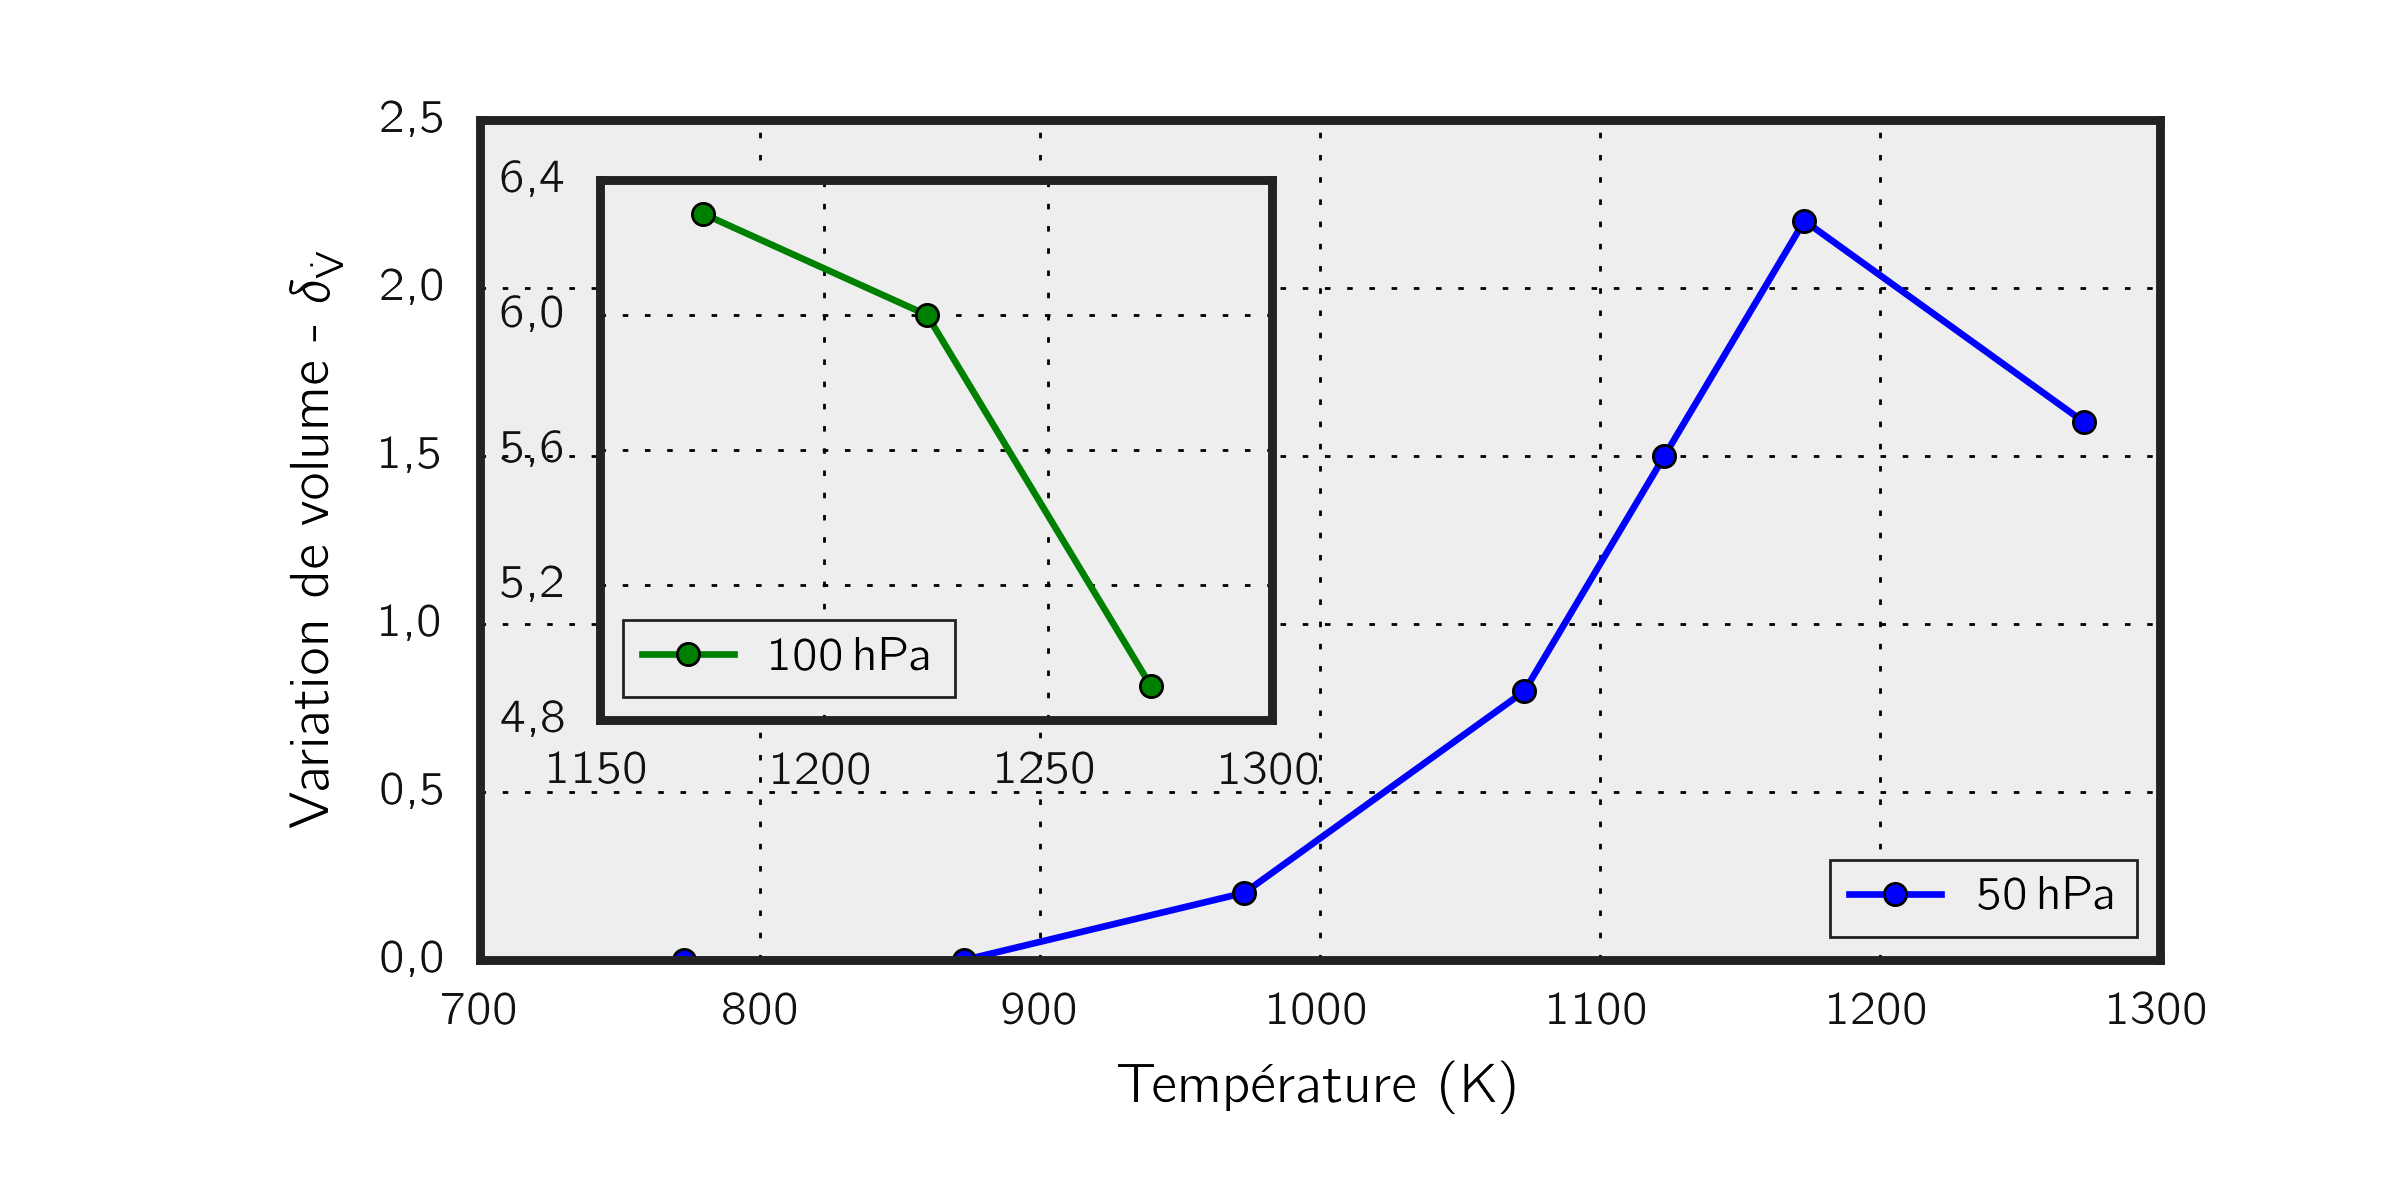
\includegraphics{figures/ch-05-kinetics-plug-flow-del-volume}}
  }\\
  \subfloat[\label{fig:plug-flow-mw-a}Masse molaire \textemdash{} \SI{50}{\hecto\pascal}]{
    \centering\resizebox{0.48\textwidth}{!}{%
      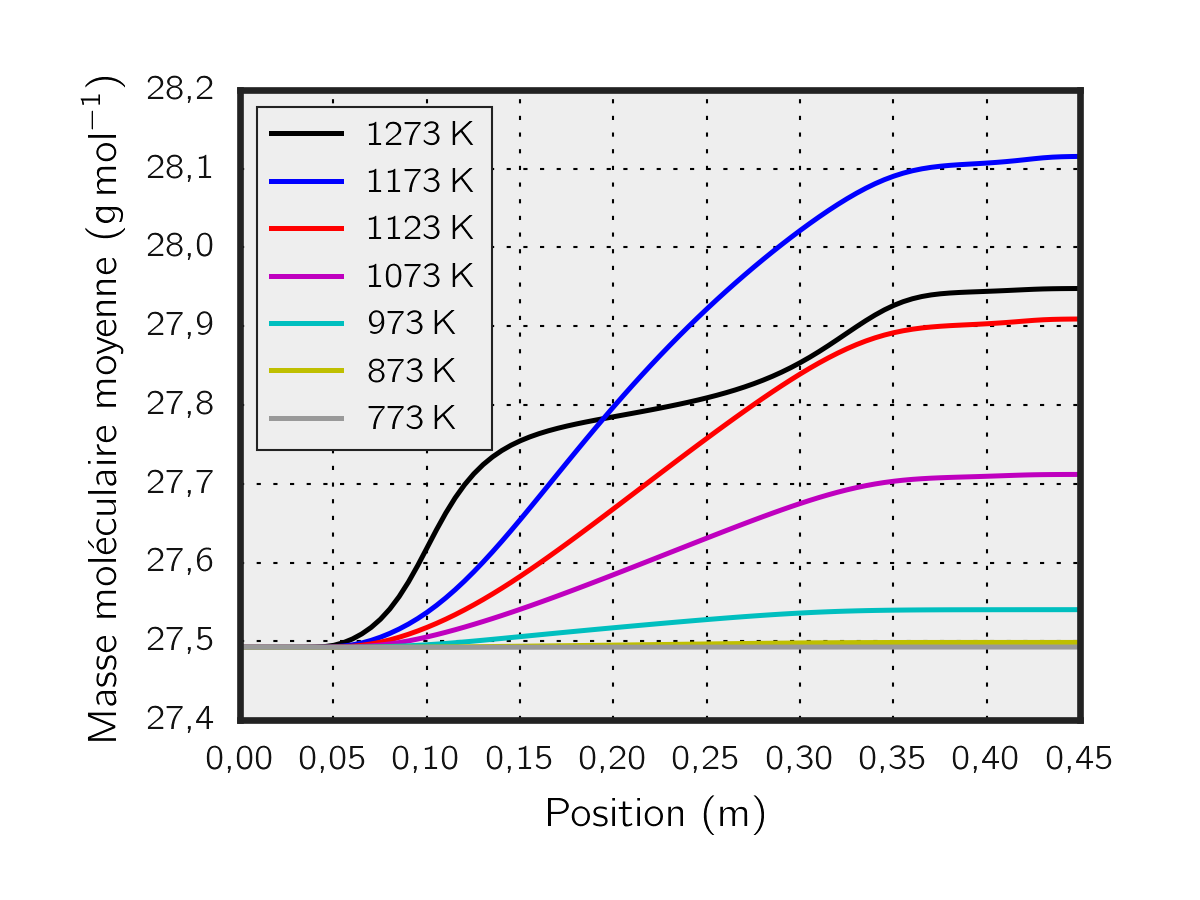
\includegraphics{figures/ch-05-kinetics-plug-flow-mw-005000Pa}}
  }\hfill
  \subfloat[\label{fig:plug-flow-mw-b}Masse molaire \textemdash{} \SI{100}{\hecto\pascal}]{
    \centering\resizebox{0.48\textwidth}{!}{%
      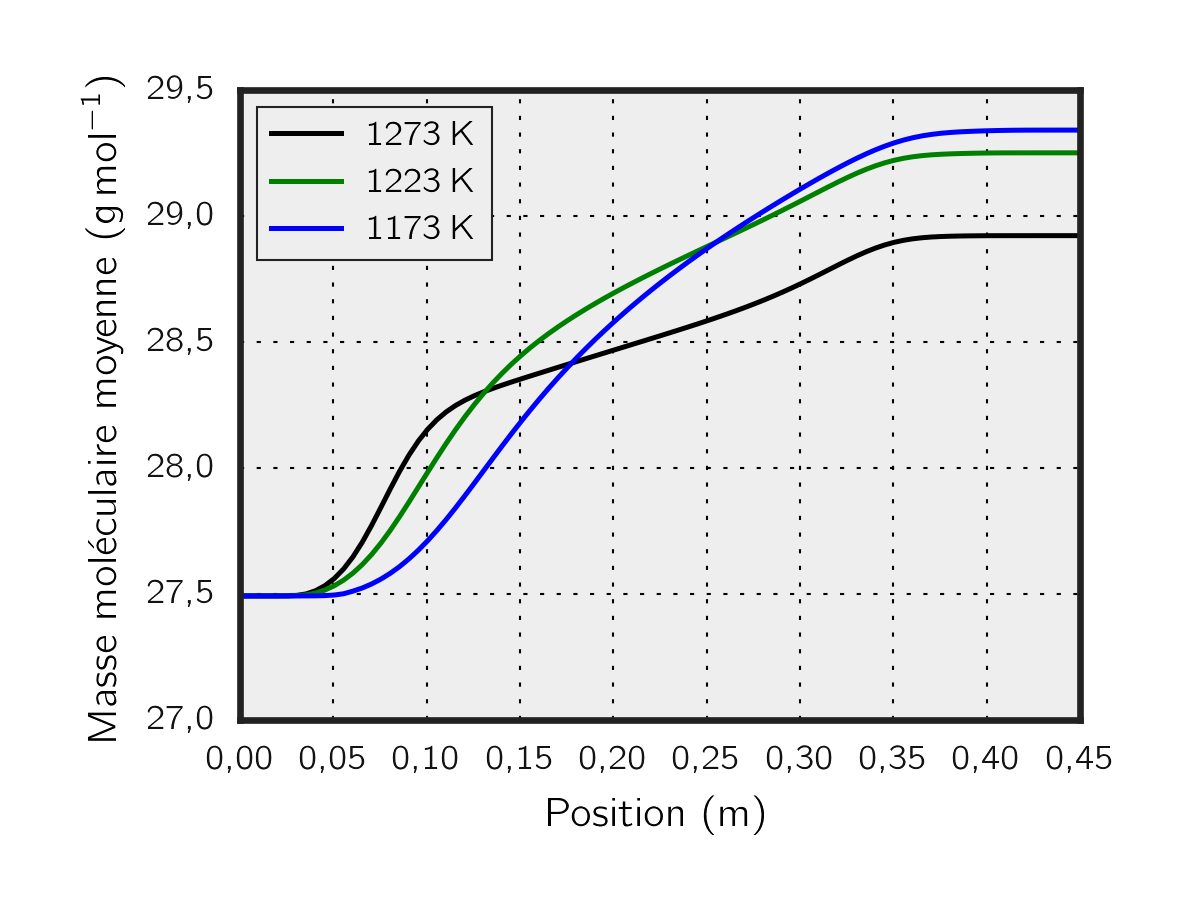
\includegraphics{figures/ch-05-kinetics-plug-flow-mw-010000Pa}}
  }
  
  \caption{Contraction du volume du gaz en fonction de la température de la zone chaude du réacteur:   \protect\subref{fig:plug-flow-del-volume} résultats à \SI{100}{\hecto\pascal} dans une fenêtre de températures réduite. Ce phénomène est associé à la masse molaire moyenne, qui est fournie en fonction de la position sur l'axe du réacteur pour différentes températures à \protect\subref{fig:plug-flow-mw-a} \SI{50}{\hecto\pascal} et à \protect\subref{fig:plug-flow-mw-b} \SI{100}{\hecto\pascal}.}
\end{figure}

\begin{figure}[!h]
  \centering
  \subfloat[\label{fig:BAPYR-low}\SI{50}{\hecto\pascal}]{
    \centering\resizebox{0.48\textwidth}{!}{%
      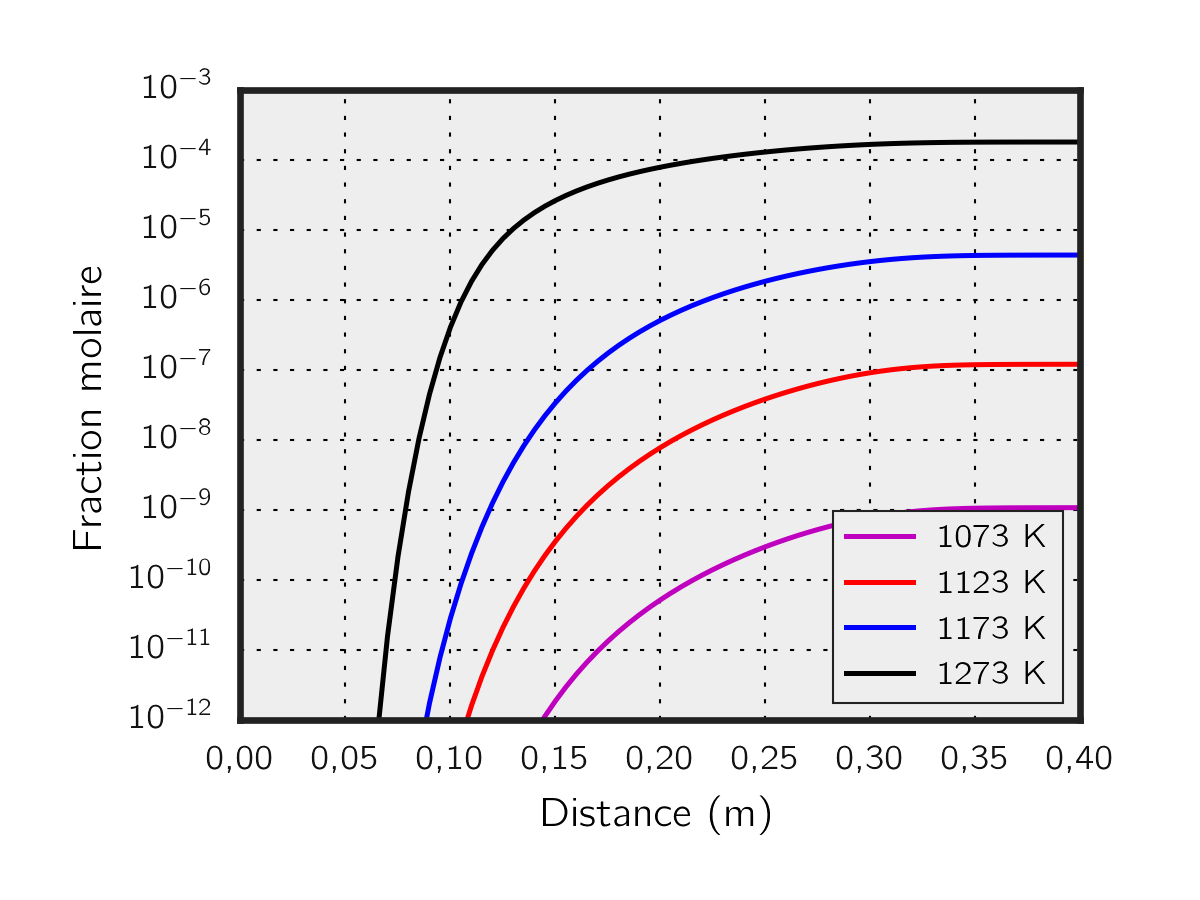
\includegraphics{figures/ch-05-kinetics-species-BAPYR-005000-Pa}}
  }\hfill
  \subfloat[\label{fig:BAPYR-high}\SI{100}{\hecto\pascal}]{
    \centering\resizebox{0.48\textwidth}{!}{%
      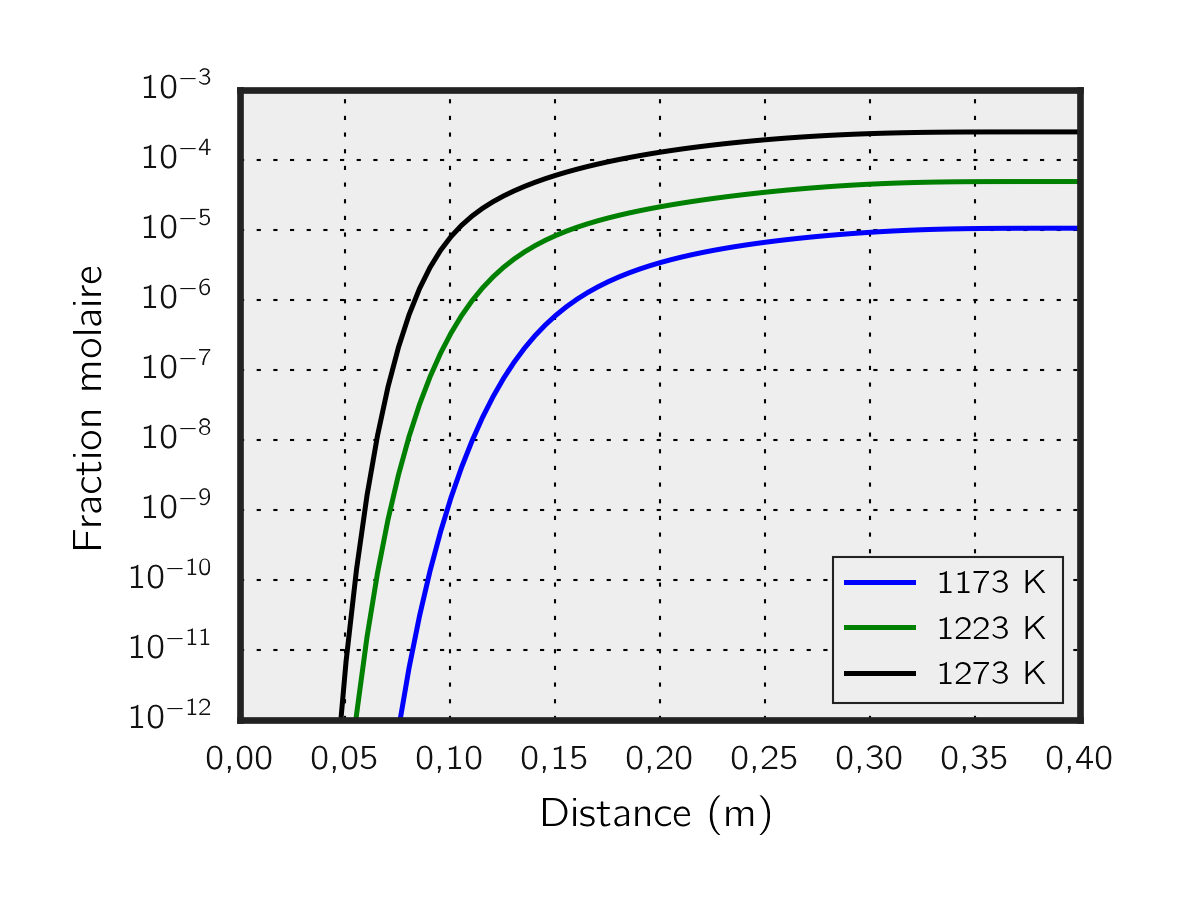
\includegraphics{figures/ch-05-kinetics-species-BAPYR-010000-Pa}}
  }
  
  \caption{\label{fig:species-BAPYR}Évolution de la fraction de benzo-a-pyrène dans la direction de l'axe du réacteur de type piston à \SIlist{50;100}{\hecto\pascal} pour une atmosphère \ch{N2 - 0,36 C2H2} à l'entrée. Simulations réalisées en utilisant le mécanisme de \citet{Norinaga2009}.}
\end{figure}

\subsection{Décomposition de l'ammoniac}
\label{sec:simulation-ammoniac-piston}

Cette section est dédiée à l'intégration des processus cinétiques relatifs à l'ammoniac dans les conditions employées expérimentalement à basse pression au Chapitre~\ref{ch:caracterisation_atmospheres}. Étant donné le fait qu'on désire intégrer les processus de surface et les échanges avec la phase gazeuse, ce qui peut conduire à la formation d'espèces atomiques~\cite{Ertl1980}, on ajoute les réactions de recombinaison de l'hydrogène et de l'azote au mécanisme de \citet{Dirtu2006}. Cette étape est nécessaire pour une future incorporation des processus détaillés dans le mécanisme de surface. Les paramètres cinétiques pour la réaction \ch{H + H <=> H2} sont fournis par \citet{Warnatz1984}, lesquels sont aussi utilisés dans les mécanismes de \citet{Norinaga2009} et \citet{AAUmech}. Pour la recombinaison de l'azote selon \ch{N + N <=> N2}, des données fournies par \citet{Clyne1967} sont incorporées au mécanisme. Le Tableau~\ref{tab:ammonia-decomposition-simulation} présente les résultats des simulations réalisées à l'aide de la version modifiée du mécanisme de \citet{Dirtu2006} dans la colonne notée \og{}Homogène\fg{}. Les profils de température le long de la zone chaude du réacteur et rapportés Section~\ref{sec:simulation-acetylene-piston} ont aussi été utilisés dans ces simulations. On observe un très mauvais accord entre les mesures expérimentales et les valeurs simulées: les processus de surface sur \ch{SiO2} jouent un rôle non-négligeable sur la décomposition de \ch{NH3}. 

Les simulations \og{}1\fg{} et \og{}2\fg{} représentent la condition de mise au point de la nitruration avec le réacteur non-chargé, pour laquelle aucune décomposition n'a été mise en évidence expérimentalement. L'incorporation d'un processus global de surface tel que proposé par \citet{Cooper1988} aux simulations, conduit aux résultats présentés sur la colonne \og{}Hétérogène\fg{}. Après introduction de la réaction globale \ch{NH3 + Qz -> 1/2 N2 + 3/2 H2 + Qz} \textendash{} où \ch{Qz} désigne un site de réaction sur les parois en quartz du réacteur \textendash{} on vérifie que pour les conditions \og{}1\fg{} et \og{}2\fg{}, aucune décomposition importante n'est observée, en accord avec les expériences. La réduction du débit dans les conditions de \og{}3\fg{} à \og{}6\fg{} conduit à des décompositions qui suivent la séquence expérimentale. Les simulations s'avèrent être en bon accord avec les expériences réalisées à \SI{1173}{\kelvin}, alors qu'un accord numérique n'a pas pu être trouvé à \SI{1073}{\kelvin}, en dehors de la plage de températures étudiée par \citet{Cooper1988}. Quelques remarques sont nécessaires: le taux de réaction global fourni par \citet{Cooper1988} est représenté par un processus de premier ordre (et supposé tel cas vérifiant l'approche de Langmuir-Hinshelwood) et aucune densité de sites réactionnels n'est fournie. Cantera~\cite{Cantera2014} requiert l'utilisation de données pour les processus élémentaires. Cela a été contourné en supposant une densité de sites égale à \SI{1,7e-9}{\mole\per\square\centi\metre}~\cite{Tang20151161} et une constante cinétique donnée par l'Équation~\ref{eq:rate-ammonia-quartz}, dont on a conservé l'énergie d'activation proposée par \citet{Cooper1988}.

\begin{equation}
  k{}={}2,71{}\times{}10^{14}{}\exp\biggr(\frac{149\si{\kilo\joule\per\mole}}{RT}\biggr)
  \quad\si{\per\second}
  \label{eq:rate-ammonia-quartz}
\end{equation}

L'incorporation des processus de surface pour des parois métalliques n'a pas été possible en raison des données fournies par \citet{Ertl1980,Arabczyk1999} qui considèrent la catalyse par le fer CC pur. Une description des processus cinétiques en domaine \ch{Fe-$\gamma$} n'a pas été trouvée dans la littérature. \citet{Bell2016} rapportent un changement de l'étape limitant la décomposition de \ch{NH3} par la désorption de \ch{N_s} \textendash{} décomposition des nitrures de fer formés en surface \textendash{} et à la scission des liaisons \ch{N-H} à haute température. Le bilan énergétique de ces transformations est simulé par \citet{Lanzani20106571}, mais aucun paramètre cinétique n'est fourni. L'Annexe~\ref{an:mécanisme-odochian} compile le mécanisme et les données thermodynamiques nécessaires aux simulations de décomposition de l'ammoniac.

\begin{table}[h]
  \caption{\label{tab:ammonia-decomposition-simulation}Simulations de la décomposition de \ch{NH3} selon le mécanisme cinétique proposé par \citet{Dirtu2006} et modifié avec nos données.}
  
  \centering{}\footnotesize{}%
  \begin{tabular}{\$c^c^c^c^c^c^c^c^c^c}
    \toprule[2pt]
    \rowstyle{\bfseries}
    \multirow{2}{*}[-3pt]{N}        &
    {Dilution}                      &
    {P}                             &
    {Q}                             &
    {T}                             &
    {$\tau_{\mathbf{eff}}$}         &
    {$S_{c}$}                       &
    \multicolumn{3}{c}{\bfseries Fraction molaire en \ch{NH3}}
    \tabularnewline
    \cmidrule{8-10} 
    &                           
    {x(\ch{NH3})}               &  
    {\si{\hecto\pascal}}        &
    {\si{\sccm}}                & 
    {\si{\kelvin}}              & 
    {\si{\second}}              &
    {\si{\square\centi\metre}}  & 
    {Mesures}                   &
    {Homogène}                  &
    {Hétérogène}
    \tabularnewline
    \midrule[2pt]
    1 & 0,25 &  50 & 684 & 1173 & 0,396 & 0,0 & 0,250 & 0,250 & 0,244
    \tabularnewline[3pt]
    2 & 0,64 &  50 & 737 & 1173 & 0,369 & 0,0 & 0,640 & 0,640 & 0,622
    \tabularnewline[3pt]
    3 & 0,98 &  50 & 470 & 1073 & 0,613 & 0,0 & 0,951 & 0,980 & 0,965
    \tabularnewline[3pt]
    4 & 0,98 &  50 & 470 & 1173 & 0,571 & 0,0 & 0,920 & 0,979 & 0,925
    \tabularnewline[3pt]
    5 & 0,98 & 100 & 470 & 1073 & 1,248 & 0,0 & 0,927 & 0,979 & 0,950
    \tabularnewline[3pt]
    6 & 0,98 & 100 & 470 & 1173 & 1,151 & 0,0 & 0,875 & 0,938 & 0,875
    \tabularnewline[3pt]
    7 & 0,23 & 100 & 687 & 1173 & - & 8,80 & 0,193 & - & -
    \tabularnewline[3pt]
    8 & 0,64 & 100 & 737 & 1173 & - & 9,54 & 0,413 & - & -
    \tabularnewline[3pt]
    9 & 0,64 & 100 & 737 & 1173 & - & 18,1 & 0,391 & - & -
    \tabularnewline
    \bottomrule    
  \end{tabular}  
\end{table}

\clearpage\section{Conclusion}

La Partie~\ref{part:part_3} de cette thèse traite de la modélisation et de la simulation des atmosphères pour les traitements thermochimiques à partir de mélanges contenant du \ch{C2H2} et du \ch{NH3}. De manière plus spécifique, nous avons choisi des mécanismes et écrit des modèles pour reproduire numériquement les expériences réalisées au Chapitre~\ref{ch:caracterisation_atmospheres}. Au cours de ce chapitre nous avons obtenu les résultats suivants:
\begin{itemize}
  \item des approches simplifiées ont été proposées pour la modélisation des réacteurs de géométrie simple. Cela a permis d'intégrer la cinétique de décomposition des précurseurs mesurée au Chapitre~\ref{ch:caracterisation_atmospheres} sans faire appel à des méthodes numériques de type CFD pour le calcul de la dynamique des fluides;
  
  \item les mécanismes pertinents de décomposition de l'acétylène et de l'ammoniac ont été sélectionnés. Le mécanisme de \citet{Norinaga2009} s'avère pertinent pour la pyrolyse des hydrocarbures \ch{C2} et plus particulièrement le \ch{C2H2}. Il a été analysé d'un point de vue topologique pour identifier les espèces les plus importantes de la décomposition de l'acétylène. La cinétique de décomposition de \ch{NH3} à basse pression s'avère beaucoup moins rapide et l'intégration des processus sur les parois en quartz du réacteur a été nécessaire en complément du mécanisme proposé par \citet{Dirtu2006}.
  
  \item l'application de la méthode de \citet{Lu2005} a été utilisée pour simplifier le mécanisme de \citet{Norinaga2009} qui s'avère trop complexe pour des simulations d'écoulements réactifs détaillés. L'utilisation de la méthode a permis l'obtention d'un mécanisme à 40 espèces \textendash{} au lieu de 241 au départ \textendash{} pour une utilisation à \SI{1173}{\kelvin} dans la plage de pressions partielles en \ch{C2H2} comprise entre \SIlist{10;40}{\hecto\pascal};
  
  \item des constantes globales ont été établies dans le cas de la pyrolyse de l'acétylène à pression atmosphérique avec des temps de séjour de l'ordre de \SI{200}{\second} et à basse pression. Les ordres de réaction ajustés avec des valeurs de $n\geq{}2$ sont en accord avec le processus principal du mécanisme global proposé par \citet{Norinaga2005}, à savoir la condensation \ch{3 C2H2 -> C6H6}; 
  
  \item les simulations des expériences à basse pression à partir de l'acétylène avec le mécanisme de \citet{Norinaga2009} se trouvent être en bon accord avec les données du Chapitre~\ref{ch:caracterisation_atmospheres}. L'écart entre les mesures de \ch{C2H2} résiduel et les valeurs simulées reste généralement inférieur à 3\%;
  
  \item les mécanismes de décomposition de l'ammoniac rapportés dans la littérature sont insuffisants pour simuler des processus en phase gazeuse avec des temps de séjour réduits. L'introduction d'une réaction globale de craquage de \ch{NH3} sur les parois en quartz du réacteur a permis de décrire la conversion hétérogène de ce précurseur à \SI{1173}{\kelvin}.
\end{itemize}

%Les bilans matière de la phase gazeuse de ces traitements sont présentés Figure~\ref{fig:bilan_matiere_nitruration_bp} avec le taux de conversion d'ammoniac calculé. Une forte consommation de \ch{NH3} est observée au début du traitement de nitruration, ce qui est lié plutôt à l'état de surface des pièces traitées et l'absence de nitrures précipités.  Cette consommation est décroissante au cours du traitement et l'état stationnaire est rapproché au but d'un certain instant. Le temps caractéristique pour atteindre cet état stationnaire est une fonction de la surface des pièces traités, comme on verra par la suite.

%La réaction globale de nitruration (Équation \ref{eq:reaction_nitruration}) peut être formulé de manière à incorporer le transfert de masse à l'état solide. En utilisant les fractions injeté et mesuré d'ammoniac le taux de conversion $\alpha$ peut être calculé numériquement en utilisant des prises de masse simulées qui conduisent à celles du Tableau \ref{tab:nitruration_bp} au but de l'enrichissement. Cela c'est fait en utilisant l'Équation \ref{eq:conversion_corrigee_etat_solid}, qui permet de rélier la composition de l'atmosphère (fraction molaire en ammoniac à l'entrée $x_{\mathrm{NH_{3}}}^{i}$ et à la sortie $x_{\mathrm{NH_{3}}}^{o}$) et le facteur d'éfficacité de nitruration $x$ au taux de conversion $\alpha$ de l'ammoniac. La Figure \ref{fig:facteur_de_nitruration} présente la valeur de $x$ au cours du traitement. Le point à l'instant initial n'est pas presenté dans la figure pour des raisons de lisibilité et vaut 0,55 pour une fraction en ammoniac de 0,64 à l'entrée et 0,66 pour une fraction de 0,23 \footnote{Ces valeurs sont absolus et pas normalisées par rapport aux surfaces traités}. Cette quantité répresente la fraction de l'ammoniac decomposé qui a apporté matière au solide et, donc, la vitesse relative de la réaction de nitruration par rapport à celle de craquage catalytique de l'ammoniac sur le surface de l'alliage traité.

%\begin{equation}
%\mathrm{NH_{3}}\stackrel{S}{\longrightarrow}\frac{1}{2}\left(1-x\right)\,\mathrm{N_{2}^{\left(g\right)}}+x\mathrm{\,N^{\left(s\right)}+\frac{3}{2}\,\mathrm{H_{2}}}\label{eq:reaction_nitruration}
%\end{equation}
%
%\begin{equation}
%\alpha=\frac{1-\nicefrac{x_{\mathrm{NH_{3}}}^{o}}{x_{\mathrm{NH_{3}}}^{i}}}{1+x_{\mathrm{NH_{3}}}^{o}\left(1-\nicefrac{1}{2}x\right)}\label{eq:conversion_corrigee_etat_solid}
%\end{equation}

%\begin{figure}
%  \begin{centering}
%    \hfill\subfloat[Facteur de nitruration.]{\begin{centering}
%        \includegraphics[scale=0.6]{figures/nitriding_factor/figure}
%        \par\end{centering}
%    }\hfill\subfloat[Vitesse de décomposition du $\mathrm{NH_{3}}$.]{\begin{centering}
%      \includegraphics[scale=0.6]{figures/nitriding_rate_global/figure}
%      \par\end{centering}
%  }\hfill
%  \par\end{centering}
%\caption{\label{fig:facteur_de_nitruration}Bilan matière de la nitruration
%  austénitique.}
%\end{figure}

%Si l'on suppose homogénéité dans l'atmosphère autour des pièces traités, i.e. que les produits en sortie représentent la comportement moyen des surfaces des échantillons, et en négligeant le changement de volume du gaz donnée la réaction de décomposition de l'ammoniac, le taux de la réaction globale de nitruration peut être approximé Équation \ref{eq:ammonia_decomposition_rate}. Les bilans matière de la Figure \ref{fig:bilan_matiere_nitruration_bp} permet donc le calcul de la vitesse de décomposition de l'ammoniac (Figure \ref{fig:facteur_de_nitruration}-b).  Les courbes ainsi tracés montrent l'effet de l'action de masse sur la cinétique de décomposition de l'ammoniac, tel que initialement attendu.

%\begin{equation}
%\frac{\mathrm{d}N_{\mathrm{NH_{3}}}}{\mathrm{d}t}=kc_{\mathrm{NH_{3}}}^{i}\left(1-\theta\right)S\label{eq:ammonia_decomposition_rate}
%\end{equation}
\endinput